\documentclass[a4paper,11pt]{report}
%\usepackage[none]{hyphenat}

%\usepackage[T1]{fontenc}
%\usepackage[bitstream-charter]{mathdesign}

%\usepackage[usenames,dvipsnames,pdf]{pstricks}
%\usepackage[crop=off]{auto-pst-pdf}
\usepackage{makeidx}
\usepackage{url}
\usepackage[square,sort,comma,numbers]{natbib}
\usepackage{framed}

\usepackage{graphicx}
\usepackage{longtable}
\usepackage{amsfonts}
\usepackage{amsmath}
\usepackage{float}

\usepackage{tabularx} % Add this to your preamble
\usepackage{booktabs} % Recommended for professional tables
\usepackage{xcolor}
\usepackage{pgfgantt}
\usepackage{tikz}
\usetikzlibrary{positioning, arrows.meta, calc, fit, backgrounds, shapes.geometric}

\usepackage{listings}
\definecolor{lstkeyword}{RGB}{0,90,160}
\definecolor{lstcomment}{RGB}{100,110,120}
\definecolor{lststring}{RGB}{160,60,40}
\definecolor{lstframe}{RGB}{200,205,210}
\lstset{
  language=Python,
  basicstyle=\ttfamily\footnotesize,
  keywordstyle=\color{lstkeyword}\bfseries,
  commentstyle=\color{lstcomment}\itshape,
  stringstyle=\color{lststring},
  numbers=left,
  numberstyle=\ttfamily\scriptsize\color{lstcomment},
  numbersep=8pt,
  frame=single,
  rulecolor=\color{lstframe},
  framexleftmargin=4pt,
  xleftmargin=16pt,
  breaklines=true,
  breakatwhitespace=true,
  showstringspaces=false,
  columns=fullflexible,
  keepspaces=true,
  captionpos=b,
  float=false,
  aboveskip=1.2em,
  belowskip=1.2em,
  emph={torch,nn,np,qmc},
  emphstyle=\color{lstkeyword}
}
\setcounter{topnumber}{4}
\setcounter{bottomnumber}{3}
\setcounter{totalnumber}{8}

\renewcommand{\topfraction}{0.92}

\renewcommand{\bottomfraction}{0.85}

\renewcommand{\textfraction}{0.06}

\renewcommand{\floatpagefraction}{0.75}
\renewcommand{\lstlistingname}{Listing}
\AtBeginDocument{\counterwithin{lstlisting}{chapter}}

\usepackage[noend,ruled,noline,linesnumbered,algochapter]{algorithm2e}

\usepackage[linktoc=page]{hyperref}
\usepackage[margin=3cm]{geometry}
\usepackage{setspace} 

\usepackage{fancyhdr}

\usepackage{parskip}
\pagestyle{fancy}

\rhead{\nouppercase\leftmark}
\lhead{\nouppercase\rightmark}

\makeindex

\onehalfspacing 

\renewcommand*\contentsname{Table of Contents}

\begin{document}

\pagenumbering{roman}

%title page
\begin{titlepage}


\begin{center}
\line(1,0){430}\\
%{ \Huge \bf Heuristically Guided\\ Local Search for \\ Protein Structure Prediction \\}
{\Huge \bf Solving the Lorenz ODE System Using Optimal ANN Architectures\\ \vspace{.5em}}
\line(1,0){430}

\end{center}

\vfill

\begin{center}
By
\end{center}


\vfill
\begin{center}

{\large \bf Ikramul Hasan Moral (0112230489)}\\[10pt]
{\large \bf Md. Abu Bakar (0112230200)}\\[10pt]
{\large \bf Samiur Rahman Omlan (0112230195)}\\[10pt]
{\large \bf Fariha Islam (0112230431)}\\[10pt]
{\large \bf Md. Touhidul Islam (0112230435)}\\

\end{center}



\vfill


\begin{center}
{Submitted in partial fulfilment of the requirements \\of the degree of Bachelor of Science in Computer Science and Engineering}
\end{center}

\vfill
\begin{center}
{\today}
\end{center}

\vfill
	
\begin{center}

\includegraphics[scale=0.15]{./uiu}
\end{center}

\begin{center}
	\textsc{Department of Computer Science and Engineering\\
		United International University}
\end{center}



\end{titlepage}



%\clearpage
%\thispagestyle{empty}
%\mbox{}
\clearpage

%\thispagestyle{empty}
%Dedication
%I would like to dedicate this thesis to my loving family ...
    



%\clearpage
%\thispagestyle{empty}
%\mbox{}
%\clearpage
%\thispagestyle{empty}
\pagenumbering{roman}
\setcounter{page}{1}


%Abstract
\setlength{\headheight}{14pt}
\begin{center}
	{\huge \bf Abstract}
	\line(1,0){430}
\end{center}
In physical modeling, nonlinear coupled ordinary differential equations (ODEs) are frequently encountered. It is not possible to obtain their analytical solutions. In most cases, the traditional approach to solving such problems is numerical methods such as the Runge-Kutta family, which comes with a computational burden and mesh-dependency. The Lorenz ODE system is a simplified meteorological model that is used as a test case in this study. This study investigates whether a standard artificial neural network (ANN), without physics-informed loss functions or operator learning configurations, can approximate the solution to this coupled system. Accurate reference data are generated using the Runge-Kutta method and the SciPy solver. Several feedforward ANN structures are then trained on this reference data. Then, change the network structure by adjusting the number of hidden layers, the number of neurons per layer, and the activation functions. Lastly, test the models by checking the mean squared error (MSE), training convergence, and the time required to compute them.

\clearpage
\setlength{\headheight}{12pt}

\begin{center}
{\huge \bf Acknowledgements}
\line(1,0){430}
\end{center}


First of all thanks to ALMIGHTY ALLAH for giving us the strength and ability to complete this project successfully.

We sincerely express our gratitude to our honorable mentor, Dr. Muhammad Nomani Kabir, Professor, Department of CSE, United International University, for his guidance, support, and encouragement throughout this project.

We also thank our respected course teacher, Dr. Md. Motaharul Islam, Professor, Department of CSE, United International University, for his kindness and valuable teachings.

We are also grateful to all the faculty members who supported and guided us in completing this project.

Last but not the least, we thank our parents and family members for their constant support, love, and encouragement.



\input{0.3.pub.tex}






\clearpage
\phantomsection
\tableofcontents
\renewcommand{\contentsname}{Table of Contents}
\addcontentsline{toc}{chapter}{Table of Contents}

\clearpage
\phantomsection
\addcontentsline{toc}{chapter}{List of Figures}
\listoffigures

\clearpage
\phantomsection
\addcontentsline{toc}{chapter}{List of Tables}
\listoftables



\clearpage
\pagenumbering{arabic}
\setcounter{page}{1}

\renewcommand\bibname{References}

\clearpage
\phantomsection


\chapter{Introduction}

This chapter introduces the research topic, provides an overview and motivation for the study, and outlines the main objectives and expected outcomes. It also outlines the methodology and briefly describes how the rest of the report is organized.

\section{Project Overview}
Ordinary Differential Equations (ODEs) describe how a system change with over time. They are widely used in fields such as physics, engineering, and mathematics. In many 
real-world problems, particularly those involving complex or nonlinear equations, it is often 
not possible to obtain exact solutions. That is why methods such as Euler’s method and 
Runge-Kutta are used to obtain approximate solutions. In this project, we examine a 
particular system consisting of three nonlinear equations known as the Lorenz-1960 system 
(one of the first meteorological models). The system is small, but complex enough to 
make a good testing ground for various solution methods. The Lorenz-1960 system is a 
great candidate for evaluating how well  artificial neural network (ANN) learn and predict behavior. Classical 
numerical methods address these problems step by step. Also they are typically accurate, but 
they are very slow and require more computational cost. We use numerical methods like Runge-Kutta to generate data that can be used to train artificial neural networks to learn how variables change over time.
The ANN learns to match its predictions with the results of the numerical solver during training. After training, the ANN can quickly predict results for any time without solving the equations again.
Therefore, the primary aim  of this project is to solve the Lorenz-1960 system 
and to see how well a plain ANN can learn its behavior and which ANN architecture provides
optimal results. 

\begin{figure}[ht]
    \centering
    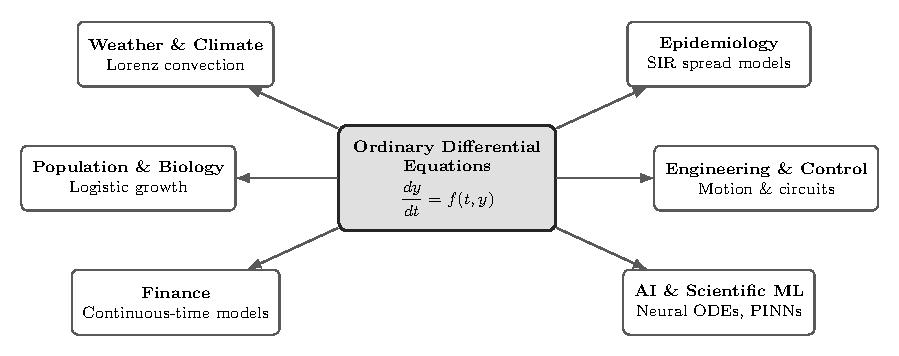
\includegraphics[width=0.9\textwidth]{ode_landscape.pdf}
    \caption{ODEs model how systems evolve over time in science, engineering, and AI.}
    \label{fig:ode_landscape}
\end{figure}


\section{Motivation}
This project is research and application driven. Classic numerical methods have been tested and proven to be accurate and reliable. They work well for directly simulating equations. A trained artificial neural network (ANN), on the other hand, can solve the equation on its own. It forecasts and behaves as a copy of the actual system. Numerous investigations are currently used: Solving differential equations with neural network approximators based on PINNs, operator learning and ANN. This makes the topic interesting and relevant to investigate. Another motivation for this project is the learning and hands-on benefits it offers. It offers the building of skills in solving an ordinary differential equation(ODEs). It also provides training on how to construct and utilize models of the neural network. The project involves running experiments and analysing results. It's useful to compare different methods. Although simple ANNs are not as powerful as advanced methods, they will give us some insights into their abilities and limitations.

\begin{figure}[ht]
    \centering
    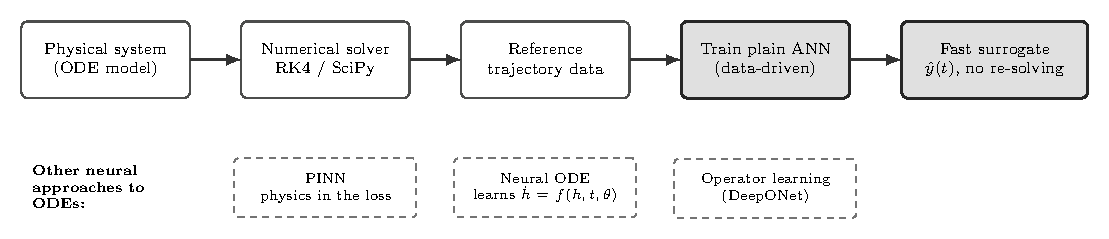
\includegraphics[width=\textwidth]{ode_in_ai.pdf}
    \caption{Neural networks learn from numerical solutions to provide fast approximations of ODE systems.}
    \label{fig:ode_in_ai}
\end{figure}

\section{Objectives}
The main aims of this project are:


\begin{itemize}
    \item  To numerically solve a coupled and nonlinear system (Lorenz equation).

\end{itemize}

\begin{itemize}
    \item To apply ODE concepts, numerical methods such as the Runge-Kutta and SciPy solvers, The Lorenz equations are solved using an ANN. Numerical solutions obtained from the Runge-Kutta method.


\end{itemize}

\begin{itemize}
    \item To generate accurate data with the Runge-Kutta method and then verify the numerical solutions with it. Compare and evaluate the performance of ANN.
    
\end{itemize}

\begin{itemize}
    \item To compare the different ANN architecture to varying the number of layers, varying number of neurons per layer and testing various activation functions to determine the most optimum one.

\end{itemize}

\begin{itemize}
    \item To evaluate the model’s performance we are using mean squared error, learning stability, and other measures, we assessed the performance of the model. See if a plain ANN can learn the Lorenz equation and explore the trade off between the two variables, namely computational cost.

\end{itemize}

\begin{itemize}
    \item To compare the results with PINN based methods from other research to understand how this approach performs compared to recent techniques.
\end{itemize}


\section{Methodology}
The “Waterfall Methodology” is being followed. Here, the various phases are carried out one after the other in a fixed order. It is fitting as we know what we want and need from the outset. In this, the input of each step is the output of the next step. This helps the process to be structured, easy to track and easy to manage.
       
       
       
       In the Literature Review phase the Lorenz-1960 equation and its property was studied.
Brief review of numerical methods, such as RK4, SciPy solvers. Besides, a number of ANN architectures, activation functions and training techniques were also investigated.
     
      
      
      The problem of the study and the objectives of the study were well stated in the Concept Development phase. The configuration of the layers in the ANNs was focused on approximation of the Lorenz-1960 equation, and the number of neurons, activation functions, learning rates and epochs of training were selected. Data sets for training and validation were prepared. 
      
      
      During the Design phase, ANN models and training strategy were developed, such as data processing and optimization of the network structure. The RK4 and SciPy were used to calculate a numerical baseline to compare with. Assessment measures, visualization tools, and statistical tests were set up to guarantee a valid comparison of models. Some statistical tests were also outlined to ensure appropriate comparisons between models. 
      
      
      During the Implementation phase numerical solvers and ANN models were developed. All of the models were trained using the datasets generated. The accuracy, training time, parameters number and convergence was measured. Each model was performed systematically based on the design. 
      
      In the Testing phase, we then tested the performance of each ANN model and then predicted
The results obtained by using the mean square error to evaluate its performance. We tested for generalization with new data. Compared the sensitivity of the models to various parameter values. The best models were compared with results from published studies. 


  Lastly, we have the Deployment phase, during which we incorporated all the results, plots, and analyses in the final project report. We designed and documented the code so that it was easy to repeat our work. The instructions for repeat experiments and retraining the models were included. We also presented our final suggestions on the best ANN architecture. This phase ensures that the project is complete and ready.
  




For better understanding, a diagram of our methodology is given below:-


\begin{figure}[h]
    \centering
    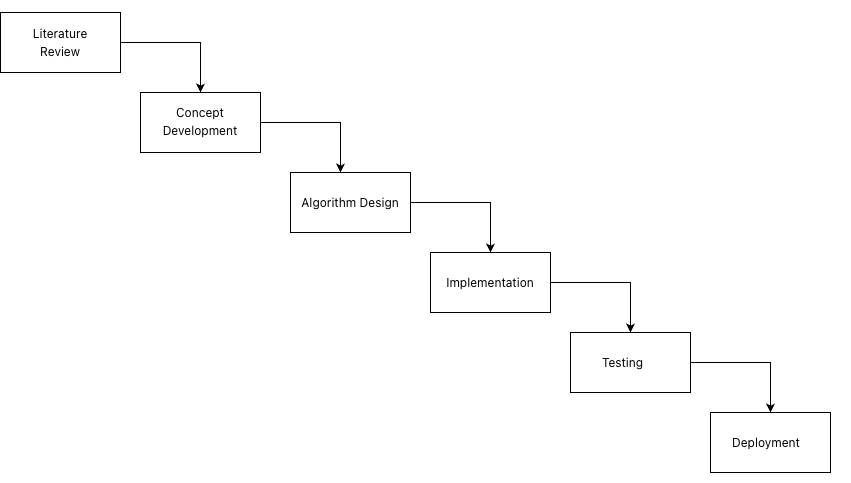
\includegraphics[width=0.8\textwidth]{Methodology.png}
    \caption{Methodology Diagram}
    \label{fig:methodology}
\end{figure}


\section{Project Outcome}
The expected outcome of the project will be the clear and the justified 
determination of the most appropriate architecture for the ANN in estimating 
the solution to the Lorenz-1960 system of ODEs within the scope of the experiment. This project must also include a 
numerical reference solution to the ODEs, the establishment of ANN 
baselines, and a comparative analysis of the results. \\[1pt]

The project will also contribute to the current understanding of the capacity
and limitations of ANN models in the approximation and solution of differential 
equations. If the ANN models are able to get a satisfactory level of accuracy in 
approximating the solution to the ODEs, the project will have demonstrated 
the capability of a simple ANN architecture to effectively act as an alternative 
numerical solver. This would suggest that a plain ANN, without the need for 
physics-informed loss terms or traditional mesh-dependent numerical 
methods, can on its own approximate ODE solutions with sufficient accuracy 
while being computationally less expensive in terms of inference time and the 
avoidance of iterative re-solving for each query. If the models do not achieve satisfactory accuracy in approximating solutions to the ordinary differential equations (ODEs), the study will clearly delineate the limitations of simple ANN architectures and mention the necessity for more advanced methods. \\[1pt]

This project will not only focus on coding and experiments, but also on understanding how different ANN structures, such as depth, width, and activation functions, influence the accuracy of solving coupled nonlinear ODE systems.



\section{Organization of the Report}
The rest of this report is outlined as follows. Chapter 2 outlines the theoretical 
background and literature review on Ordinary Differential Equations (ODE) 
solving, artificial neural networks, and existing neural methods for differential 
equations. Chapter 3 discusses about the project design, requirements, 
methodological plan, and task assignment. Chapter 4 outlines the 
implementation \& experiment design used in this research. Chapter 5 outlines 
the results and analysis on the tested ANN structures. Finally, Chapter 6 
concludes this report by focusing the main results, limitations, and potential 
directions for the future research. 

\chapter{Background}

This chapter covers the foundational knowledge you need to understand our work. We start with the mathematical and computational preliminaries. Then we review the existing literature on ANN-based ODE solvers and similar applications. We identify the research gaps that motivate our study. Finally, we wrap up with a brief summary.

\section{Preliminaries}

This section provides the necessary background knowledge to understand the rest of the report.

\subsection{Ordinary Differential Equations}

An ODE describes how a quantity changes with respect to a single independent variable. A general first-order ODE takes the form:

\begin{equation}
\frac{dy}{dt} = f(t, y), \quad y(t_0) = y_0
\label{eq:first_order_ode}
\end{equation}

where $y(t)$ is the unknown function, $t$ is the independent variable, and $y_0$ is the initial condition.

\subsection{The Lorenz-1960 System}

The Lorenz-1960 system \cite{lorenz1960max} consists of three coupled nonlinear ODEs for meteorological modeling. We target the formulation from \cite{matthews2024pinnde} (Section 4.2):

\begin{equation}
\begin{aligned}
\frac{dx}{dt} &= kl\left(\frac{1}{k^2 + l^2} - \frac{1}{k^2}\right) yz \\
\frac{dy}{dt} &= kl\left(\frac{1}{l^2} - \frac{1}{k^2 + l^2}\right) xz \\
\frac{dz}{dt} &= \frac{kl^2}{2}\left(\frac{1}{k^2} - \frac{1}{l^2}\right) xy
\end{aligned}
\label{eq:lorenz1960}
\end{equation}

with $k = 2$, $l = 1$, initial conditions $x(0) = 0.5$, $y(0) = 0.75$, $z(0) = 1$, and $t \in [0, 1]$. Its nonlinear, coupled dynamics make it an excellent benchmark for numerical solvers.

\subsection{Classical Numerical Methods}

Euler's method approximates the solution via a first-order Taylor expansion:
\begin{equation}
y_{n+1} = y_n + h \cdot f(t_n, y_n)
\end{equation}
where $h$ is the step size. It is simple but accumulates errors quickly.

The fourth-order Runge-Kutta method (RK4) evaluates the derivative at multiple points per step for higher accuracy:
\begin{equation}
y_{n+1} = y_n + \frac{h}{6}(k_1 + 2k_2 + 2k_3 + k_4)
\end{equation}

Both methods are mesh-dependent, require re-solving for every new initial condition, and struggle with stiff equations.

\subsection{Artificial Neural Networks}

A feedforward ANN (Multilayer Perceptron) consists of an input layer, hidden layers, and an output layer. Each neuron computes:

\begin{equation}
a_i(\mathbf{x}) = \sigma\left(\mathbf{w}^{(i)} \cdot \mathbf{x} + b^{(i)}\right)
\label{eq:neuron}
\end{equation}

where $\mathbf{w}^{(i)}$ are weights, $b^{(i)}$ is bias, and $\sigma$ is an activation function \cite{lau2020oden}. The Universal Approximation Theorem \cite{lau2020oden, babni2025error, hornik1989multilayer} guarantees that a network with at least one hidden layer can approximate any continuous function to arbitrary accuracy. Common activation functions include:
\begin{itemize}
    \item \textbf{Sigmoid}: $\sigma(x) = \frac{1}{1 + e^{-x}}$, maps inputs to $(0, 1)$
    \item \textbf{Tanh}: $\sigma(x) = \frac{e^x - e^{-x}}{e^x + e^{-x}}$, maps inputs to $(-1, 1)$
    \item \textbf{ReLU}: $\sigma(x) = \max(0, x)$, efficient but non-smooth at zero
    \item \textbf{GELU/Swish}: smooth ReLU approximations with better gradient flow
\end{itemize}

Training minimizes a loss function $L(\theta)$ over network parameters $\theta$ using gradient descent. Backpropagation computes gradients via the chain rule, and optimizers like Adam adapt learning rates per parameter \cite{dubey2024solving, audu2026neural}.

\subsection{ANN-Based ODE Solving}

Instead of stepping through the domain, ANNs learn a continuous solution function over the entire domain. The standard approach \cite{lagaris1998ann, mall2013comparison, okereke2021novel} constructs a trial solution:

\begin{equation}
\psi_t(x, \mathbf{p}) = A(x) + F(x, N(x, \mathbf{p}))
\label{eq:trial_solution}
\end{equation}

where $A(x)$ satisfies the initial/boundary conditions exactly, and $N(x, \mathbf{p})$ is the neural network output. The loss function measures how well this trial solution satisfies the ODE:

\begin{equation}
L(\mathbf{p}) = \frac{1}{N} \sum_{i=1}^{N} \left[ \frac{d\psi_t(x_i, \mathbf{p})}{dx} - f(x_i, \psi_t(x_i, \mathbf{p})) \right]^2
\label{eq:ode_loss}
\end{equation}

Minimizing this loss yields a differentiable, closed-form approximate solution without requiring knowledge of the exact answer.

\subsection{Physics-Informed Neural Networks}

PINNs embed governing equations directly into the loss function \cite{raissi2019pinn, matthews2024pinnde, babni2025error, audu2026neural}:

\begin{equation}
L(\theta) = L_{\text{data}} + \lambda_1 L_{\text{physics}} + \lambda_2 L_{\text{IC/BC}}
\end{equation}

The physics loss uses automatic differentiation to compute derivatives of the network output. This enables training with sparse or no data, but balancing the loss terms requires careful hyperparameter tuning.

\subsection{Network Architectures}

To better understand the differences in methodology, we present the standard architectures used in recent studies. Figure~\ref{fig:ann_arch} illustrates a typical Artificial Neural Network (ANN) architecture used for predicting system parameters without physics-informed constraints \cite{Bre}. This standard feedforward structure relies entirely on data-driven learning through backpropagation.

\begin{figure}[H]
    \centering
    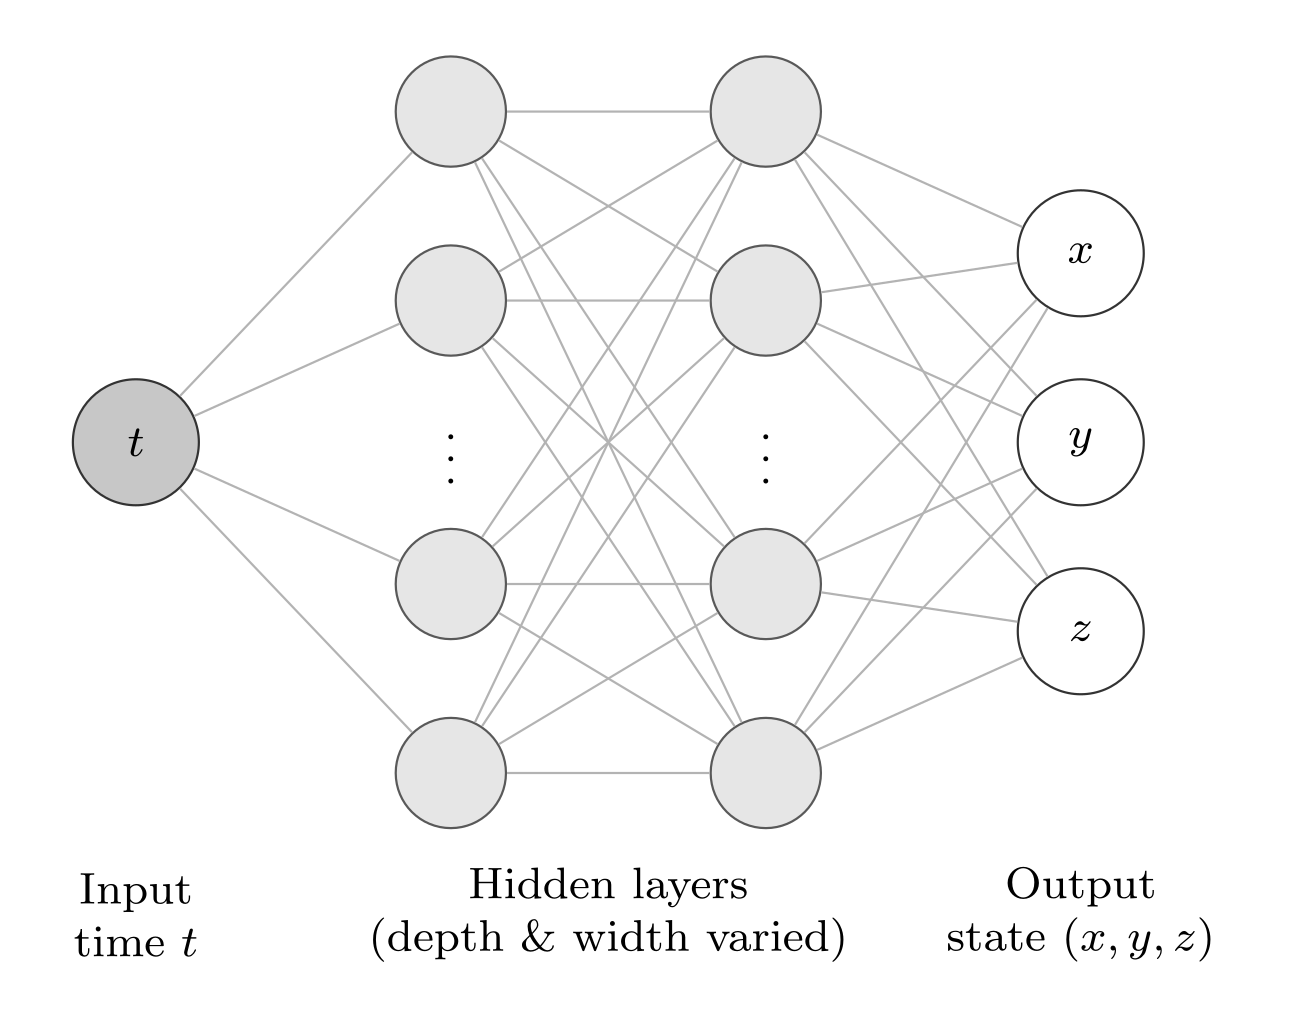
\includegraphics[width=0.85\textwidth]{ann_architecture.png}
    \caption{Typical Artificial Neural Network architecture \cite{Bre}.}
    \label{fig:ann_arch}
\end{figure}

In contrast, Figure~\ref{fig:pinn_arch} demonstrates a Physics-Informed Neural Network (PINN) architecture. In this approach, the standard ANN output is further constrained by physical laws---specifically, the governing differential equations of the system---which are embedded directly into the loss function \cite{Zhai}.

\begin{figure}[H]
    \centering
    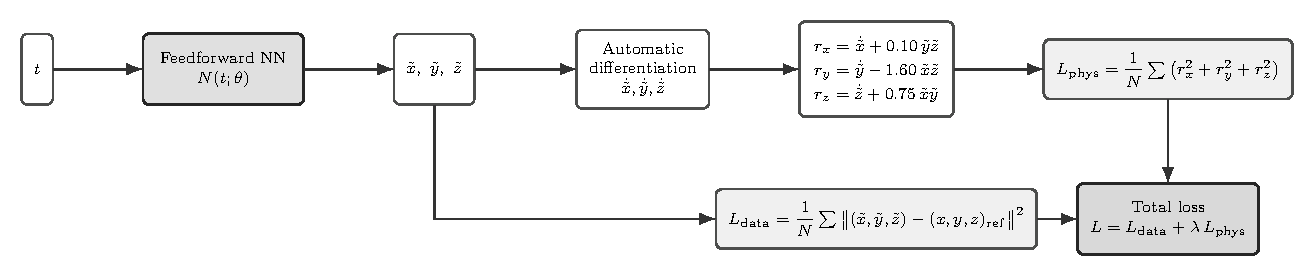
\includegraphics[width=\textwidth]{pinn_architecture.pdf}
    \caption{Architecture of a Physics-Informed Neural Network incorporating physical loss \cite{Zhai}.}
    \label{fig:pinn_arch}
\end{figure}


\section{Literature Review}

\subsection{Similar Applications}

Dubey et al. \cite{dubey2024solving} used an ANN (tanh activation) to solve coupled first-order ODEs with an error of $2.88 \times 10^{-3}$ in a maximum of 120 iterations. A comparable PyTorch-based ANN was used by Audu et al. \cite{audu2024utilizing}, which converged in 200--1500 iterations. Okereke et al. \cite{okereke2021novel} bypassed backpropagation by calculating the weights based on regression with Gaussian Radial Basis Functions. The ODEN framework developed by Lau and Werth \cite{lau2020oden} demonstrates that NNs outperform RK4 on rapidly oscillating solutions, with errors of $\sim 10^{-4}$. On a damped vibration equation, Mall and Chakraverty \cite{mall2013comparison} compared arbitrary versus regression-based weight initialization and they found that regression-based weights reduce maximum deviation from 3.67\% to 1.47\%. Murugesh et al. \cite{murugesh2025novel} used neural networks with block numerical methods to directly solve higher-order ODEs and obtaining errors near machine precision ($\sim 10^{-10}$). Pratama et al. \cite{pratama2022ann} surveyed three ANN-based PDE solvers (PyDEns, NeuroDiffEq, Nangs) and used 3 hidden layers with 32 neurons and tanh activation. NeuroDiffEq uses the Trial Approximate Solution methodology, which suggests that initial conditions are hardcoded in the ansatz. This is a pure ANN method that is applied to our research.


\subsection{Related Research}

\subsubsection{Physics-Informed Approaches}

PinnDE was proposed by Matthews and Bihlo \cite{matthews2024pinnde}, which solved the Lorenz-1960 system using a DeepONet (4 hidden layers, 40 nodes, tanh, Adam optimizer). Their DeepONet is trained to learn the operator $G(u_0)(t, x)$ which provides solutions given initial conditions over $[0, 1]$. This is the closest baseline to our target problem, but it relies on physics-informed loss terms. Babni et al. \cite{babni2025error} generalized the trial construction $\tilde{u}(x, \theta) = P(x) + Q(x)N(x, \theta)$ by replacing $Q(x)$ with a flexible $\varphi(x)$, proving the error bound $|N_\varphi(t, \theta) - u(t)| \leq e^{\kappa|t - t_0|} L_\varphi(\theta)$. This verifies that the smaller the loss, the smaller the solution error. Audu et al. \cite{audu2026neural} compared PINN and ANN models using six first-order ODE tests. Their PINN had an error of $10^{-8}$ to $10^{-10}$ which was much better as compared to ANN. This raises the issue of whether architecture optimization can bridge this gap or not.

\subsubsection{Pure ANN Approaches}

The NeuroDiffEq Trial Approximate Solution is physics-free. Pratama et al. \cite{pratama2022ann} found that NeuroDiffEq can train without physics loss terms which is consistent with our methodology. But they benchmarked only on the heat equation which is linear. Dubey et al. \cite{dubey2024solving} claim that plain ANNs can solve coupled ODEs but used a fixed architecture. Okereke et al. \cite{okereke2021novel} removed backpropagation through weight computation instead of polynomial fitting. Audu et al. \cite{audu2024utilizing} achieved an error of $10^{-4}$ with a sigmoid ANN on three first-order ODEs. All these studies do not examine the implications of building patterns on performance.

\subsubsection{Architecture and Loss Function Studies}

Mall and Chakraverty \cite{mall2013comparison} made comparisons between 4, 5, and 6 hidden nodes with random and regression-based weights. Weights that are based on regression are always better compared to random weights. After 6 nodes they found that accuracy remains the same. They applied only sigmoid activation on simple ODEs. Lau and Werth \cite{lau2020oden} discovered that sigmoid / tanh need less training in comparison to ReLU / ELU. Xavier initialization speeds up the convergence and Adam is better than SGD. They did not vary systematically depth and width. Xiong \cite{xiong2022new} arranged seven constructions (polynomial, exponential, hyperbolic, logarithmic, logistic, sigmoid, softplus) of loss functions. Exponential is best when applied to the law of Newton cooling and logarithmic is best when it is applied to the motor suspension system.

\subsubsection{Lorenz System Studies}

Aslam et al. \cite{aslam2024neuro} have used ANN + PSO-NNA hybrid optimization to solve Lorenz equations (Neurons=10, sigmoid, N=90, independent runs=100). They are directed to a diverse Lorenz parameterization ($\sigma, \rho, \beta$), are based on meta heuristic optimization and do not compare architectures.

\subsubsection{Neural ODEs}

Chen et al. \cite{chen2018neural} proposed neural ODEs where the derivative function $\frac{dh(t)}{dt} = f(h(t), t, \theta)$ that is parameterized with a neural network and trained using the adjoint method efficient for backpropagation. This sample is quite different than ours where we learn the dynamics ($f$) while neural ODEs find the approximation of the solution ($y(t)$) itself.

\subsubsection{Hybrid Approaches}

Murugesh et al. \cite{murugesh2025novel} proposed a Neural-ODE Hybrid Block Method with the update rule:

\begin{equation}
y(t_{k+1}) = y(t_k) + h \sum_{j=0}^{m-1} \omega_j f_\theta(t_{k-j}, y_{k-j}) + \sum_{i=0}^{m-1} \alpha_i F(t_{k-i}, y_{k-i})
\end{equation}

where $\omega_j$ and $\alpha_j$ balance neural versus numerical contributions. It achieved machine-precision errors on harmonic oscillators and the Van der Pol equation.

\clearpage % Ensures we start at the top of a fresh page so we have maximum room

\section{Gap Analysis}

Table~\ref{tab:gap_analysis_updated} summarizes what each reviewed paper covers and where gaps exist.

\vspace{-1em} % Pulls the table up slightly closer to the text

\begin{table}[!ht] % Using !ht is safer and won't crash your document
    \centering
    \caption{Comprehensive Literature Gap Analysis}
    \label{tab:gap_analysis_updated}
    \tiny % Using \tiny ensures the table is physically short enough to share the page with your list
    \renewcommand{\arraystretch}{1.0} 
    \setlength{\tabcolsep}{2pt} % Shrinks padding to fit text better
    
    \begin{tabularx}{\textwidth}{| 
        >{\hsize=0.6\hsize\raggedright\arraybackslash}X | 
        >{\hsize=1.15\hsize\raggedright\arraybackslash}X | 
        >{\hsize=1.15\hsize\raggedright\arraybackslash}X | 
        >{\hsize=1.05\hsize\raggedright\arraybackslash}X | 
        >{\hsize=1.05\hsize\raggedright\arraybackslash}X | 
        >{\hsize=1.0\hsize\raggedright\arraybackslash}X |
        }
        \hline
        \textbf{Paper} & \textbf{Methodological Approach} & \textbf{Target Differential Equations} & \textbf{Architectural Investigation} & \textbf{Lorenz-1960 Application} & \textbf{Plain ANN Implementation} \\
        \hline
        
        \cite{matthews2024pinnde} & PINN + DeepONet: Integrates physics laws and operator networks into the loss function. & Solves both ODEs and PDEs using governing physics. & No systematic study of network structural impact. & Evaluated specifically as a complex dynamical system. & Uses physics-informed logic, not a plain ANN. \\
        \hline
        
        \cite{pratama2022ann} & PyDEns / ANN: Standard networks for field estimation. & Primary focus on solving Partial Differential Equations (PDEs). & General overview without specific layer/neuron testing. & The study does not address the Lorenz model. & Covers standard ANN architectures for PDEs. \\
        \hline
        
        \cite{chen2018neural} & Neural ODE: Derivative represented as a neural network. & Models continuous-time dynamics for ODEs. & Focuses on functional flexibility, not structural depth. & Not specifically tested on the Lorenz system. & Relies on specialized ODE-solver integration. \\
        \hline
        
        \cite{aslam2024neuro} & ANN + PSO-NNA: ANN with Particle Swarm Optimization. & Applied to solving Ordinary Differential Equations. & Optimization focuses on weights, not architectural depth. & Directly applied to Lorenz-based chaotic dynamics. & Uses heuristic optimization instead of plain training. \\
        \hline
        
        \cite{lau2020oden} & Plain ANN: Standard feedforward network approach. & General application for approximating ODE solutions. & Provides a limited (partial) study on hidden layers. & Tested on other benchmarks, not Lorenz-1960. & Utilizes a standard, plain ANN configuration. \\
        \hline
        
        \cite{mall2013comparison} & ANN: Implementation of neural networks for equations. & Targets solutions for ODEs in engineering. & Includes a detailed study on network architecture. & Application restricted to simpler, non-chaotic ODEs. & Employs a basic feedforward ANN structure. \\
        \hline
        
        \cite{xiong2022new} & ANN: Simple neural solver for dynamic systems. & Focused on solving Ordinary Differential Equations. & Does not explore the impact of different layer counts. & Does not address the chaotic Lorenz-1960 model. & Uses a traditional, data-driven ANN model. \\
        \hline
        
        \cite{babni2025error} & PINN: Physics-Informed Neural Networks approach. & Solves ODEs by embedding equations in the loss function. & No investigation into depth or width performance. & Not applied to the meteorological Lorenz model. & Strictly uses physics-informed constraints. \\
        \hline
        
        \cite{dubey2024solving} & Plain ANN: Feedforward network trained on numerical data. & Applied to various Ordinary Differential Equations. & Lacks a systematic study of network architecture. & No specific testing on the Lorenz system. & Uses a standard numerical data training pipeline. \\
        \hline
        
        \cite{okereke2021novel} & ANN: Basic neural network models for ODEs. & Aimed at solving standard ODE systems. & Does not perform structural performance analysis. & No mention or testing of the Lorenz-1960 system. & Follows a traditional, plain ANN approach. \\
        \hline
        
        \cite{audu2024utilizing} & Plain ANN: Usage for initial value problems in ODEs. & Specifically handles ODE solution approximation. & No detailed evaluation of layers or neurons. & Focused on other common types of ODEs. & Relies on a standard feedforward structure. \\
        \hline
        
        \cite{audu2026neural} & PINN vs ANN: A comparative study of two methods. & Analysis restricted to Ordinary Differential Equations. & Lacks an in-depth architecture comparison study. & Not applied to the Lorenz-1960 model. & Discusses ANN only in comparison to PINN. \\
        \hline
        
        \cite{murugesh2025novel} & Hybrid: Combines different neural modeling techniques. & Solves ODEs using integrated hybrid approaches. & Architecture optimization is not the primary focus. & Does not utilize the Lorenz-1960 test case. & Incorporates external optimization methods. \\
        \hline

        \cite{lagaris1998ann} & ANN: Trial-solution method using a feedforward network. & Solves ODEs, ODE systems, and PDEs. & No systematic study of layers or neurons. & Does not test the Lorenz-1960 system. & Plain feedforward ANN trained on the ODE residual. \\
        \hline

        \cite{raissi2019pinn} & PINN: Embeds governing equations in the loss function. & Targets forward and inverse nonlinear PDEs. & No systematic study of depth or width. & Not applied to the Lorenz-1960 model. & Uses physics-informed constraints, not a plain ANN. \\
        \hline

        \cite{lorenz1960max} & Analytical: Reduces the vorticity equation to three ODEs. & Derives the coupled nonlinear Lorenz-1960 ODEs. & Predates neural network architecture studies. & Defines the original Lorenz-1960 system. & Uses no neural network of any kind. \\
        \hline

        \cite{hornik1989multilayer} & Theory: Proves the universal approximation property. & Not concerned with differential equations. & Shows one hidden layer suffices for approximation. & Does not address the Lorenz-1960 system. & Covers feedforward networks in general, not a solver. \\
        \hline

        \textbf{Our Work} & \textbf{Plain ANN: Traditional feedforward network.} & \textbf{Direct solution of coupled ODE systems.} & \textbf{Comprehensive study of hidden layers and density.} & \textbf{Primary test case for predicting chaotic dynamics.} & \textbf{Purely data-driven ANN without physics aids.} \\
        \hline
        
    \end{tabularx}
\end{table}

The literature review reveals five specific gaps that our research addresses:

\begin{enumerate}
    \item \textbf{No architecture study for the Lorenz-1960 system:} Matthews and Bihlo \cite{matthews2024pinnde} solve the Lorenz-1960 system but use a fixed DeepONet architecture without optimization. Aslam et al. \cite{aslam2024neuro} study a different Lorenz parameterization. No existing paper systematically compares ANN architectures on the Lorenz-1960 system.

    \item \textbf{No PINN vs. plain ANN comparison on Lorenz-1960:} Audu et al. \cite{audu2026neural} compared PINN and ANN on simple first-order ODEs. No study makes this comparison on a nonlinear, coupled ODE system like Lorenz-1960.

    \item \textbf{No systematic activation function study for ODE solving:} Pratama et al. \cite{pratama2022ann} use tanh throughout without ablation. Lau and Werth \cite{lau2020oden} note that sigmoid and tanh outperform ReLU but do not test modern alternatives like GELU or Swish. Mall and Chakraverty \cite{mall2013comparison} use only sigmoid. No study compares activation functions (tanh, ReLU, sigmoid, GELU, Swish) on a coupled ODE system.

    \item \textbf{No systematic depth and width study for ODE solution quality:} Mall and Chakraverty \cite{mall2013comparison} test 4, 5, and 6 nodes on simple ODEs. Lau and Werth \cite{lau2020oden} observe that architecture should match equation complexity. But no paper systematically varies both depth (2--6 layers) and width (20--100 neurons) to find the optimal configuration for a Lorenz-type system.

    \item \textbf{Limited generalization studies:} Most papers train for a single initial condition. The ability to generalize across different initial conditions remains largely unexplored for coupled nonlinear ODE systems.
\end{enumerate}

Our research fills these gaps by performing a systematic architecture comparison on the Lorenz-1960 ODE system using plain ANNs. We vary depth, width, and activation functions while benchmarking against RK4 reference solutions and the PINN-based results from Matthews and Bihlo \cite{matthews2024pinnde}.


\section{Summary}

This chapter established the necessary background for our research. We reviewed the mathematical foundations of ODEs, the Lorenz-1960 system, classical numerical methods, and ANN-based solving approaches. The literature review covered 17 research papers spanning physics-informed methods, pure ANN approaches, architecture studies, Lorenz system solvers, Neural ODEs, and hybrid techniques.

The gap analysis reveals that no existing study performs a systematic architecture comparison of plain ANNs on the Lorenz-1960 ODE system. Existing works either use fixed architectures, focus on simpler equations, or rely on physics-informed loss terms. Our research directly addresses this gap by varying network depth, width, and activation functions to identify the optimal ANN architecture for solving the Lorenz-1960 system as an initial value problem.

The next chapter presents our project design, including the detailed methodology, experimental setup, and evaluation plan.


\chapter{Project Design}

In this chapter, we describe the design of the experiment. This chapter will be the
requirements of our pipeline needs to meet also the context it operates in. The two-phase
methodology used for the architecture search and optimizer comparison.


\section{Requirement Analysis}

We have a clear set of requirements for our pipeline. It should have certain outputs and has defined quality.
Set goals and work within a set of limits. This is a computing research project,
Not a software product is. Thus, the requirements are towards reproducibility, numerical accuracy,
and disciplined experimentation.

\subsection{Functional and Nonfunctional Requirements}

The functional requirements describe the actions that the pipeline performs in each phase. Beginning at the pipeline's creation
the reference solution to producing the final comparison report. The nonfunctional requirements determine the quality level. There are two strict requirements – reproducibility and reference accuracy.

\begin{table}[H]
\centering
\caption{Functional Requirements of the Research Pipeline}
\label{tab:fr}
\renewcommand{\arraystretch}{1.2}
\begin{tabular}{|p{1.2cm}|p{12.5cm}|}
\hline
\textbf{ID} & \textbf{Requirement} \\
\hline
FR1 & The system shall be required to generate a high-accuracy numerical reference solution for The Lorenz-1960 ODE system using the fourth-order Runge-Kutta and the SciPy library, evaluated over the interval $t \in [0, 1]$ at $1001$ uniformly spaced points. \\
\hline
FR2 & The system shall partition the reference dataset into training and validation subsets using 80/20 random split with a fixed random seed. \\
\hline
FR3 & The system shall construct feedforward ANN models with systematically varied parameters.
These parameters include depth (1 to 4 hidden layers), width (20, 50, or 100 neurons per layer),
and activation function (tanh, ReLU, sigmoid, GELU, or Swish). \\
\hline
FR4 & The system shall train all Phase 1 models under identical conditions using the Adam optimizer and record convergence behaviour for each run. \\
\hline
FR5 & The system shall conduct a Phase 2 optimizer comparison using the three best Phase 1 architectures.
Each architecture will be trained with Adam, L-BFGS, and SGD with mo momentum.mentum.
momentum. \\
\hline
FR6 & The system shall evaluate each trained model using MSE, MAE, maximum absolute error, training time, and inference time against the RK4 reference. \\
\hline
FR7 & The system shall produce comparison tables, solution trajectory plots, and error curves for every evaluated models. \\
\hline
\end{tabular}
\end{table}

\begin{table}[H]
\centering
\caption{Nonfunctional Requirements of the Research Pipeline}
\label{tab:nfr}
\renewcommand{\arraystretch}{1.2}
\begin{tabular}{|p{1.5cm}|p{12.2cm}|}
\hline
\textbf{ID} & \textbf{Requirement} \\
\hline
NFR1 & All experiments shall be fully reproducible using a single fixed random seed applied to weight initialization and data splitting. \\
\hline
NFR2 & The numerical reference solution shall maintain solver agreement of RMSE below $10^{-10}$ between the custom RK4 implementation and SciPy. \\
\hline
NFR3 & All results, model configurations, and metrics shall be logged systematically so that an independent reader can verify the reported findings. \\
\hline
\end{tabular}
\end{table}

\subsection{Context Diagram}

Figure~\ref{fig:context} shows the research pipeline as one bounded system with two external entities.
The first is a research team. We set up experiments and start them as well as gather the results.
the resulting models and metrics. The second are the academic and research community.
They eat the reported results, repeat the approach and extend the comparisons.
results. Each internal process such as reference generation, final reporting, and so on resides within the
pipeline. There are no other living processes outside the system boundary.


\begin{figure}[H]
\centering
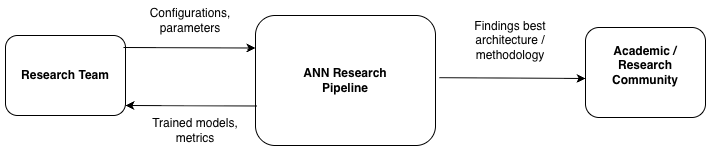
\includegraphics[width=0.85\textwidth]{context_diagram.png}
\caption{Context diagram of the research pipeline.}
\label{fig:context}
\end{figure}

\subsection{Data Flow Diagram Level 1}

Figure~\ref{fig:dfd1} divides the research pipeline into a series of five steps. Process P1 generates
Plot the reference trajectory with both the RK4- and SciPy-solvers. P2 makes it preprocess the trajectory
It is done through the 80/20 split and z-score normalization of the output targets.
P3 trains the ANN models, initially over the complete Phase 1 grid, and subsequently over the Phase 2
optimizer comparison. P4 test each of the trained models with the reference solution
using the metrics from FR6. P5 compares the results, selects the best architecture and Creates the final report.

\begin{figure}[ht]
\centering
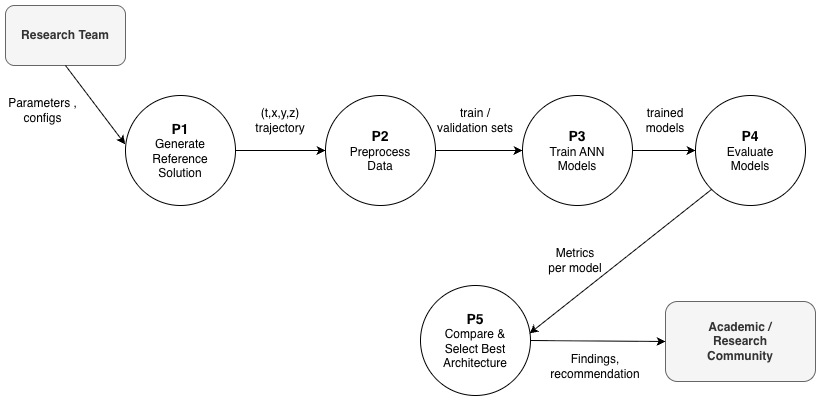
\includegraphics[width=0.95\textwidth]{dfd_level1.png}
\caption{Data Flow Diagram (Level 1) showing the five internal processes of the research pipeline.}
\label{fig:dfd1}
\end{figure}

\subsection{UI Design}

This project has no user interface. We run everything from Python scripts and Jupyter notebooks. Results are stored as figures, tables, and serialized model files. UI design does not apply here.

\section{Detailed Methodology and Design}

The methodology is divided into two phases. Here is the logic.

\begin{itemize}
    \item \textbf{Phase 1 -- Architecture Search (60 runs):} We choose the depth: 1--4 hidden layers, width: 20, 50, 100 neurons, and activation functions: tanh, ReLU, Sigmoid, GELU and Swish. Also we choose the optimizer fixed at Adam. This will show us which architectural choices matter most.
    \item \textbf{Phase 2 -- Optimizer Comparison (9 runs):} We take the three best architectures from Phase 1. Then fine-tune each one with the following three algorithms: Adam, L-BFGS, SGD with momentum. All other factors remain unchanged.All other factors remain constant. This indicates the percentage of optimization that the optimizer will use to
contributes on top of the architecture.

\end{itemize}

This separation allows that the two comparisons are not confused. If any
Improvements in Phase 2 do not result from optimizing the network, but from a change in the network structure.


\subsection{Reference Solution Generation}

We calculate the reference solution from the Lorenz-1960 system with $k=2$, $l=1$, initial conditions $x(0)=0.5$, $y(0)=0.75$, $z(0)=1$, and time interval $t \in [0, 1]$, as defined in Chapter~2. Two independent solvers are used to ensure that reference numbers are accurate. The first is a custom-made fourth-order Runge-Kutta integrator with step size $h=10^{-3}$ . Evaluated at a common grid of points $1001$ points. The second one is the solve ivp of SciPy  routine using DOP853 with $\text{rtol}=10^{-10}$ and $\text{atol}=10^{-12}$ which is sampled on the same grid. We need agreement between both solvers at RMSE below $10^{-10}$ and then we use
The RK4 trajectory was adopted as the reference trajectory for training and evaluation of all the ANNs. This dual solver are make sure to check and catch the unintentional mistakes in either implementation. Also it provides us a reliable reference and the rest of the study will be based on this.

\subsection{Dataset Preparation}

The reference trajectory provides us with $1001$ ,$(t, x(t), y(t), z(t))$. That is our training set. Our training set is 80\% training (around $800$ points) and our validation set is 20\% validation (about $201$ points) and we report our results on the validation set. The data is split randomly into two halves, with seed $42$. It comes as a surprise to us all but we do the split once before training any model. All configurations of the ANN use the same training points, validation points, and validation error.The same training points, the same validation points, and the same validation error are used in every ANN configuration.
and in the same order. 
We then normalize each of the three target variables by using the training-set,
the mean and standard deviation. Given $x$ , $y$ and $z$ , this $z$ score normalization puts $x$ , $y$ and $z$ on a comparable scale, to ensure that the loss function is not being swamped by the variable with the largest range of variation range. The key to this is that all errors are reported after unnormalisation. The published metrics stay in the original physical units of the system.


\subsection{Model Family and Architecture (Phase 1)}

Each candidate ANN is a simple feedforward network.  Accepts scalar time $t$ as an argument, it is used for predicting the three dimentional state vector $(x(t), y(t), z(t))$. The hidden structure varies with The number of hidden layers, the number of neurons in each hidden layer, activation function. We explore these values in Phase 1 as listed in Table~\ref{tab:phase1grid}. 

The Cartesian product of these axes results in $4 \times 3 \times 5 = 60$ distinct architectures. We
Optimize each one separately with the same optimization parameters. The output layer is
always linear with three units. We do not include any skip connections, normalization layers, and
no regularization. This is a simple design on purpose. It helps hold the comparison to one's mind. From our research question about the three architectural axes, the following questions were developed.


\begin{table}[H]
\centering
\caption{Phase 1 Architecture Search Grid}
\label{tab:phase1grid}
\renewcommand{\arraystretch}{1.2}
\begin{tabular}{|l|l|}
\hline
\textbf{Axis} & \textbf{Values} \\
\hline
Depth (hidden layers) & 1, 2, 3, 4 \\
\hline
Width (neurons per layer) & 20, 50, 100 \\
\hline
Activation function & tanh, ReLU, sigmoid, GELU, Swish \\
\hline
Total configurations & $4 \times 3 \times 5 = 60$ \\
\hline
\end{tabular}
\end{table}

\subsection{Optimizer Comparison (Phase 2)}

Phase 2 takes the three architectures with the lowest combined validation MSE from Phase 1 and retrains each one with two additional optimizers: L-BFGS and SGD with momentum. Everything else stays the same as Phase 1. We reuse the Adam result from Phase 1 as the third comparison point. That gives us $3 \times 3 = 9$ Phase 2 runs.

Why these optimizers? L-BFGS is a strong baseline for smooth, low-dimensional regression problems. Researchers commonly cite it as effective for ANN-based ODE solvers. SGD with momentum serves as a classical reference. This phase isolates the optimizer's effect from the network architecture's effect. This separation would not be achievable if optimizer selection were included in the Phase 1 search grid.

\subsection{Loss Function and Training Protocol}

The training loss is the mean squared error between the normalized predicted state and the normalized reference state, computed jointly over all three output components. We add no initial-condition penalty and no physics-based residual. This is consistent with the plain-ANN scope from Chapter~2 and avoids the loss-balancing problem that plagues physics-informed approaches.

Here are the training settings:

\begin{itemize}
    \item Phase 1 uses Adam with learning rate $10^{-3}$ and default momentum parameters.
    \item Each model trains for at most $10{,}000$ epochs.
    \item Early stopping monitors validation loss with a patience of $500$ epochs and restores the best-validation weights when training ends.
    \item We use full-batch gradient descent. The training set is small enough that full-batch is appropriate, and it removes minibatch noise as a confounding variable across configurations.
    \item We set the PyTorch random seed to $42$ before constructing each model, so weight initialization is reproducible too.
\end{itemize}


\subsection{Evaluation Metrics}
The results of each model trained are tested and compared with the RK4 reference result.
using 5 metrics. Table ~\ref{tab:metrics}  lists them. MSE is the major indicator as it corresponds to This training goal and allows them to compare all the configurations directly. The absolute
error and the maximum absolute error are the reported per state variable. They provide a
more comprehensible representation of the best and worst scenarios deviations. Training
time relates to the amount of the cost to train a particular architecture. Inference time
represents the cost of prediction of the complete trajectory when it is trained. Together,
These five are the indicators that will help us in our search of the accuracy/cost trade-off we're looking for our research question.

\begin{table}[H]
\centering
\caption{Evaluation Metrics Used for Each Trained Model}
\label{tab:metrics}
\renewcommand{\arraystretch}{1.2}
\begin{tabular}{|l|p{9.5cm}|}
\hline
\textbf{Metric} & \textbf{Purpose} \\
\hline
MSE (per variable and combined) & Primary loss. Consistent comparison across all $69$ runs \\
\hline
MAE (per variable) & Interpretable error magnitude in original physical units \\
\hline
Maximum absolute error & Worst-case deviation along the trajectory \\
\hline
Training time (seconds) & Computational cost of fitting a given architecture \\
\hline
Inference time (seconds) & Cost of predicting the full $1001$-point trajectory after training \\
\hline
\end{tabular}
\end{table}

\subsection{Alternative Solutions Considered}

We looked at several alternatives before settling on the plain feedforward ANN with a pure MSE loss. Here is what we rejected and why.

A PINN would re-use the hyperparameter and add a residue term to the loss.Balancing problem described in Chapter 2. It also would make it difficult to distinguish between our work The current PinnDE research and the ongoing PinnDE study. So we dropped it.

The same reason was rejected for a DeepONet operator-learning approach. PinnDE
A DeepONet is already tested by already on the same equation. The reproduction of that design would not address the architecture-selection gap that we found.


We explored the possibility of a Neural ODE formulation as it is a different paradigm. However, Neural ODEs do not parameterize the solution function, they parameterize the derivative. That does not give an answer to our research question

Lastly, we considered fusing the architecture search and an optimizer selection as a single process. We did not accept this as there would be more experiments in total. And mix the two effects we wish to separate from each other. The two phase design while still maintaining a clean attribution of the, adopted has the number of runs at 69 observed differences.

\section{Project Plan}

The project plan is a research design that is designed to be carried out over 42 weeks in the following way: FYDP-I, FYDP-II, and FYDP-III. The schedule groups the work into research and writing, baseline and data preparation, implementation, analysis and validation, presentation and The timeline is based on the sequence of submission milestones, according to the scope of the problem. Results verification, report, framing and numerical baseline validation to ANN experiments Completing and defence preparation. Each of the three phases are 14 weeks long, with the last one being a deliberate review. 2 weeks will be dedicated to each phase of the defense preparation and final presentation. The task placement is provided in Figure ~\ref{fig:fydp_gantt} and Table ~\ref{tab:gantt_task_ids} shows the placement across the three 14-week trimesters. Specifies the names in the chart.


\begin{figure}[H]
\centering
\caption{42-week FYDP Gantt chart using task IDs.}
\label{fig:fydp_gantt}
\resizebox{\textwidth}{!}{%
\begin{ganttchart}[
    hgrid,
    vgrid,
    x unit=0.28cm,
    y unit chart=0.31cm,
    bar height=0.42,
    group height=0.24,
    milestone height=0.34,
    group label font=\bfseries\tiny,
    bar label font=\bfseries\tiny,
    milestone label font=\bfseries\tiny,
    title label font=\tiny\bfseries,
    title height=0.7,
    group/.append style={fill=black!45},
    milestone/.append style={fill=red!70},
    progress label text={}
]{1}{42}
\gantttitle{FYDP-I}{14}
\gantttitle{FYDP-II}{14}
\gantttitle{FYDP-III}{14} \\
\gantttitle{1}{1}
\gantttitle{}{5}
\gantttitle{7}{1}
\gantttitle{}{5}
\gantttitle{14}{2}
\gantttitle{}{5}
\gantttitle{21}{2}
\gantttitle{}{5}
\gantttitle{28}{2}
\gantttitle{}{5}
\gantttitle{35}{2}
\gantttitle{}{5}
\gantttitle{42}{2} \\
\ganttgroup{FYDP-I}{1}{14} \\
\ganttbar[bar/.append style={fill=blue!55}]{T01}{1}{2} \\
\ganttbar[bar/.append style={fill=blue!55}]{T02}{3}{6} \\
\ganttbar[bar/.append style={fill=blue!55}]{T03}{7}{10} \\
\ganttbar[bar/.append style={fill=teal!60}]{T04}{8}{12} \\
\ganttbar[bar/.append style={fill=orange!70}]{T05}{11}{12} \\
\ganttbar[bar/.append style={fill=orange!70}]{T17}{13}{14} \\
\ganttmilestone{M01}{14} \\
\ganttgroup{FYDP-II}{15}{28} \\
\ganttbar[bar/.append style={fill=teal!60}]{T06}{15}{16} \\
\ganttbar[bar/.append style={fill=green!55}]{T07}{15}{20} \\
\ganttbar[bar/.append style={fill=green!55}]{T08}{19}{23} \\
\ganttbar[bar/.append style={fill=green!55}]{T09}{23}{25} \\
\ganttbar[bar/.append style={fill=purple!55}]{T10}{20}{26} \\
\ganttbar[bar/.append style={fill=orange!70}]{T11}{24}{26} \\
\ganttbar[bar/.append style={fill=orange!70}]{T18}{27}{28} \\
\ganttmilestone{M02}{28} \\
\ganttgroup{FYDP-III}{29}{42} \\
\ganttbar[bar/.append style={fill=purple!55}]{T12}{29}{32} \\
\ganttbar[bar/.append style={fill=purple!55}]{T13}{31}{34} \\
\ganttbar[bar/.append style={fill=blue!55}]{T14}{33}{36} \\
\ganttbar[bar/.append style={fill=blue!55}]{T15}{35}{39} \\
\ganttbar[bar/.append style={fill=orange!70}]{T16}{38}{40} \\
\ganttbar[bar/.append style={fill=orange!70}]{T19}{41}{42} \\
\ganttmilestone{M03}{42}
\end{ganttchart}%
}

\vspace{0.5em}
\scriptsize
\begin{tabular}{lll}
\textcolor{blue!70}{\rule{1em}{0.8em}} Research and writing &
\textcolor{teal!70}{\rule{1em}{0.8em}} Baseline and data &
\textcolor{green!70}{\rule{1em}{0.8em}} Implementation \\
\textcolor{purple!70}{\rule{1em}{0.8em}} Analysis and validation &
\textcolor{orange!80}{\rule{1em}{0.8em}} Presentation &
\textcolor{red!75}{\rule{1em}{0.8em}} Milestone
\end{tabular}
\end{figure}

\begin{table}[H]
\centering
\caption{Task and Milestone IDs Used in the Gantt Chart}
\label{tab:gantt_task_ids}
\scriptsize
\renewcommand{\arraystretch}{1.08}
\begin{tabularx}{\textwidth}{@{}p{0.7cm}>{\raggedright\arraybackslash}X>{\centering\arraybackslash}p{1.0cm}p{0.7cm}>{\raggedright\arraybackslash}X>{\centering\arraybackslash}p{1.0cm}@{}}
\toprule
\textbf{ID} & \textbf{Task or Milestone} & \textbf{Weeks} &
\textbf{ID} & \textbf{Task or Milestone} & \textbf{Weeks} \\
\midrule
T01 & Problem framing and objectives & 1--2 & T10 & Metrics, logging, and visualizations & 20--26 \\
T02 & Literature review and gap analysis & 3--6 & T11 & Chapter 4 draft and presentation & 24--26 \\
T03 & Requirements and standards mapping & 7--10 & T18 & Defense preparation and final presentation & 27--28 \\
T04 & Baseline validation and dataset specification & 8--12 & M02 & FYDP-II submission milestone & 28 \\
T05 & Interim report and presentation & 11--12 & T12 & Result verification and reproducibility review & 29--32 \\
T17 & Defense preparation and final presentation & 13--14 & T13 & Comparative analysis and final figures & 31--34 \\
M01 & FYDP-I submission milestone & 14 & T14 & Standards, constraints, and impact analysis & 33--36 \\
T06 & Canonical dataset generation & 15--16 & T15 & Final report revision and conclusion & 35--39 \\
T07 & ANN training pipeline implementation & 15--20 & T16 & Final presentation and defense preparation & 38--40 \\
T08 & Phase 1 architecture search & 19--23 & T19 & Defense preparation and final presentation & 41--42 \\
T09 & Phase 2 optimizer comparison & 23--25 & M03 & Final submission and defense & 42 \\
\bottomrule
\end{tabularx}
\end{table}

\section{Task Allocation}
There are 5 members in our team. We divided up tasks by skill area and also mapped all of the members' contributions to FYDP-I, FYDP-II and FYDP-III. This prevents treating the
write chapters without regard to the rest of the book. All members are involved in the same research pipeline consisting of a variety of planning to final defense with different primary ownership.


\begin{table}[H]
\centering
\caption{Task Allocation Across Team Members and FYDP Segments}
\label{tab:tasks}
\scriptsize
\renewcommand{\arraystretch}{1.2}
\begin{tabularx}{\textwidth}{|p{2.4cm}|>{\raggedright\arraybackslash}X|>{\raggedright\arraybackslash}X|>{\raggedright\arraybackslash}X|}
\hline
\textbf{Member} & \textbf{FYDP-I Responsibilities} & \textbf{FYDP-II Responsibilities} & \textbf{FYDP-III Responsibilities} \\
\hline
Ikramul Hasan Moral & Lead numerical baseline validation; verify the Lorenz-1960 equation setup; define data-generation requirements. & Implement preprocessing, model definitions, training loop, and experiment runner for the $69$ planned runs. & Recheck reproducibility, archive scripts and results, and support technical defense of the implementation. \\
\hline
Md. Abu Bakar & Support requirements analysis and metric selection; review literature related to evaluation criteria. & Build the evaluation pipeline; compute MSE, MAE, maximum error, training time, and inference time. & Consolidate final tables; verify result consistency against the requirements; support analysis discussion. \\
\hline
Samiur Rahman Omlan & Prepare methodology diagrams and initial experimental workflow documentation. & Produce convergence plots, solution trajectory plots, and architecture-comparison figures. & Finalize visual evidence for Chapter~4 and presentation slides; support result interpretation. \\
\hline
Fariha Islam & Lead literature review, gap analysis, citation tracking, and Chapters~1--2 drafting. & Maintain citation consistency while implementation details are added to Chapter~4. & Revise the final report for academic tone, citation coverage, and defense-readiness. \\
\hline
Md. Touhidul Islam & Compile Chapter~3 planning material, task allocation, and interim-report structure. & Coordinate weekly documentation, report updates, and experiment-log summaries. & Compile the final report, Chapter~5 constraints, Chapter~6 conclusion, and final presentation narrative. \\
\hline
\end{tabularx}
\end{table}

All members participate in supervisor meetings, progress journals, internal result reviews, and FYDP presentations. Shared review is necessary because an error in the solver, dataset, model configuration, or interpretation would affect the whole research conclusion.

\section{Summary}

 Chapter 1 into a conceptual framework.The research question from Chapter 1 and literature gap from Chapter 1 was transformed into a conceptual framework in this chapter. Chapter 2 into a concrete experimental design. Functional requirements tell you what the pipeline must yield and the non-functional requirements tell you the quality the pipeline must achieve. The context
The pipeline is put in its research environment by diagram and Level 1 data flow diagram.
A two-phase comparative study methodology is used. A 60-configuration phase 1 run is executed. Search over depth, width and activation function for architecture. Phase 2 is a 9 configuration optimizer comparison of the three best architectures. This means 69 controlled experiments altogether. We calculate reference data and check it on two different solvers.
We keep training, loss and evaluation settings fixed for all the runs so that they are observed . The differences are attributable to variables studied. The project plan assigns the work to the three segments of FYDP (each 14 weeks). There is a two-week period for defense preparation and the final presentation at the end of each phase. The items have been captured as tasks T17, T18 and T19 in the revised 42-week schedule. The task allocation Delegates team members to implementation, analysis and writing. In the next chapter, the implementation of this design and the experimental results from it are reported 69 runs.

\chapter{Implementation and Results}

This chapter documents the physics-informed neural network (PINN) built for the Lorenz-1960 system. It explains where the governing equations come from, traces each symbol into the source code, describes the network and its training, and reports the accuracy achieved. The entire pipeline is fundamentally built on PyTorch. The quantities that define the problem are imported from the baseline module rather than restated, so the equations exist in one place.

The method is built on stages and this chapter follows those stages in order.

\begin{table}[H]
\centering
\caption{How this chapter builds the method, stage by stage.}
\label{tab:roadmap}
\begin{spacing}{1.0}
\small
\begin{tabularx}{\textwidth}{|p{1.0cm}|>{\raggedright\arraybackslash}X|p{2.6cm}|}
\hline
\textbf{Stage} & \textbf{What it produces} & \textbf{Section} \\
\hline
1 & The problem: equations, coefficients $c$, initial state $u_0$, interval $[t_0, t_f]$ & \ref{sec:impl_equations} \\
\hline
2 & The baseline: reference trajectory $u^{\mathrm{ref}}$ & \ref{sec:impl_reference} \\
\hline
3 & The code map: modules and every symbol's definition site & \ref{sec:impl_software} \\
\hline
4 & The approximator: raw network $\mathcal{N}(t;\theta)$ & \ref{sec:impl_network} \\
\hline
5 & The trial solution $u_T(t)$, satisfying $u_T(t_0) = u_0$ by construction & \ref{sec:impl_ic} \\
\hline
6 & The residual $r(t)$: departure from the equations at one instant & \ref{sec:impl_residual} \\
\hline
7 & The collocation set $\{t_i\}_{i=1}^{N_c}$: where the residual is measured & \ref{sec:impl_collocation} \\
\hline
8 & The objective $\mathcal{L}(\theta)$ and the optimiser that minimises it & \ref{sec:impl_training} \\
\hline
9 & The measured error of the trained network against $u^{\mathrm{ref}}$ & \ref{sec:impl_results} \\
\hline
\end{tabularx}
\end{spacing}
\end{table}

\section{Governing Equations and Their Source}
\label{sec:impl_equations}

This section explains the problem and the equations on which the network is trained on. It also presents the coefficients of the Lorenz equations, the settings taken from the reference study, and the symbol mappings in the code. 


\subsection{The System and Its Coefficients}

The system consists of a Lorenz-1960 model in the form given by Matthews and Bihlo \cite{matthews2024pinnde}, Section 4.2, and reproduced as Equation~\ref{eq:lorenz1960} in Chapter~2. Parameters are general wavenumber $k$ and $l$,

\begin{equation}
\begin{aligned}
\frac{dx}{dt} &= kl\left(\frac{1}{k^2 + l^2} - \frac{1}{k^2}\right) yz, \\
\frac{dy}{dt} &= kl\left(\frac{1}{l^2} - \frac{1}{k^2 + l^2}\right) xz, \\
\frac{dz}{dt} &= \frac{kl}{2}\left(\frac{1}{k^2} - \frac{1}{l^2}\right) xy.
\end{aligned}
\label{eq:impl_lorenz_general}
\end{equation}

That reference states the system in Section 4.2 and gives code for it in Appendix A.2, and the two disagree. Section 4.2 is authoritative here. Appendix A.2 is not used.

The benchmark uses $k = 2$ and $l = 1$. Substitution gives three constants:

\begin{align}
c_x &= kl\left(\frac{1}{k^2 + l^2} - \frac{1}{k^2}\right) = 2\left(\frac{1}{5} - \frac{1}{4}\right) = -0.10, \label{eq:coeff_x}\\
c_y &= kl\left(\frac{1}{l^2} - \frac{1}{k^2 + l^2}\right) = 2\left(1 - \frac{1}{5}\right) = 1.60, \label{eq:coeff_y}\\
c_z &= \frac{kl}{2}\left(\frac{1}{k^2} - \frac{1}{l^2}\right) = 1\left(\frac{1}{4} - 1\right) = -0.75. \label{eq:coeff_z}
\end{align}

All three are exact in binary floating point. The reduced system solved by the network is therefore

\begin{equation}
\frac{dx}{dt} = -0.10\,yz, \qquad
\frac{dy}{dt} = 1.60\,xz, \qquad
\frac{dz}{dt} = -0.75\,xy.
\label{eq:impl_lorenz_reduced}
\end{equation}

The same source fixes the initial condition and the interval: $x(0) = 0.5$, $y(0) = 0.75$, $z(0) = 1$, and $t \in [0, 1]$. Writing $u = (x, y, z)$ and $u_0 = (0.5,\, 0.75,\, 1)$, the problem is the initial value problem $\dot{u} = f(u)$, $u(t_0) = u_0$, with $t_0 = 0$ and $t_f = 1$.

The coefficients are not hard-coded. The implementation calls \texttt{Lorenz-1960\_\allowbreak coefficients(k,\,l)} in the locked baseline, which evaluates Equations~\ref{eq:coeff_x}--\ref{eq:coeff_z} and returns $(-0.10,\, 1.60,\, -0.75)$. Changing $k$ or $l$ changes the equations without any edit to the network code.

\subsection{Adopted Settings and Notations}

Table~\ref{tab:adopted} separates what is taken from the reference study from what is chosen here. Section~\ref{sec:impl_comparison} returns to the differences.

\begin{table}[H]
\centering
\caption{Elements adopted from the reference study and elements chosen for this work.}
\label{tab:adopted}
\begin{spacing}{1.0}
\small
\begin{tabularx}{\textwidth}{|p{4.0cm}|>{\raggedright\arraybackslash}X|p{3.0cm}|}
\hline
\textbf{Element} & \textbf{Value} & \textbf{Source} \\
\hline
Equations, parameters, initial condition, interval & Equation~\ref{eq:impl_lorenz_general} with $k = 2$, $l = 1$; $u_0 = (0.5,\, 0.75,\, 1)$; $t \in [0, 1]$ & \cite{matthews2024pinnde}, Sec.~4.2 \\
\hline
Depth, width, activation & $4$ hidden layers of $60$ units, tanh & \cite{matthews2024pinnde}, Sec.~4.1 \\
\hline
Collocation and optimizer & $3000$ Latin hypercube points; Adam, $20{,}000$ iterations & \cite{matthews2024pinnde}, Sec.~4.1 \\
\hline
Initial-condition treatment & hard, by trial solution & this work, after \cite{lagaris1998ann} \\
\hline
Reference solver & DOP853 at $\text{rtol}=10^{-10}$ & this work \\
\hline
\end{tabularx}
\end{spacing}
\end{table}


\begin{table}[H]
\centering
\caption{Every symbol in this chapter and the code identifier that holds it.}
\label{tab:notation}
\begin{spacing}{1.0}
\small
\begin{tabularx}{\textwidth}{|p{2.9cm}|>{\raggedright\arraybackslash}X|p{4.6cm}|}
\hline
\textbf{Symbol} & \textbf{Meaning} & \textbf{Code identifier} \\
\hline
$t$ & Time, the single network input & \texttt{t} \\
\hline
$t_0 = 0$, $t_f = 1$ & Endpoints of the solution interval & \texttt{Config.t\_span} \\
\hline
$u = (x, y, z)$ & State vector & \texttt{u} \\
\hline
$u_0 = (0.5, 0.75, 1)$ & Initial state & \texttt{Config.initial\_state}, \texttt{PINN.u0} \\
\hline
$k = 2$, $l = 1$ & Wavenumbers & \texttt{Config.k}, \texttt{Config.l} \\
\hline
$c = (c_x, c_y, c_z)$ & Reduced coefficients & \texttt{lorenz1960\_coefficients} $\rightarrow$ \texttt{PINN.coeffs} \\
\hline
$f(u)$ & Right-hand side of the system & local \texttt{f} in \texttt{ode\_residual} \\
\hline
$\theta$ & Trainable parameters & \texttt{model.parameters()} \\
\hline
$\mathcal{N}(t;\theta)$ & Raw network output & \texttt{self.net(t)} \\
\hline
$L = 4$, $H = 60$ & Hidden layers, units per layer & \texttt{Config.depth}, \texttt{Config.width} \\
\hline
$g(t)$ & Ramp vanishing at $t_0$ & \texttt{g} in \texttt{PINN.forward} \\
\hline
$u_T(t)$ & Trial solution & return of \texttt{PINN.forward} \\
\hline
$r(t)$ & ODE residual & return of \texttt{residual} \\
\hline
$\{t_i\}_{i=1}^{N_c}$, $N_c = 3000$ & Collocation times & \texttt{grid}, \texttt{Config.n\_collocation} \\
\hline
$\mathcal{L}(\theta)$ & Training objective & \texttt{loss} in \texttt{train} \\
\hline
$\lambda_{\mathrm{IC}}$ & Soft-IC penalty weight, unused here & \texttt{Config.gamma} \\
\hline
$\{\tau_m\}_{m=1}^{M}$, $M = 1001$ & Evaluation times & reference grid, \texttt{n\_eval} \\
\hline
$u^{\mathrm{ref}}$ & DOP853 reference trajectory & \texttt{reference\_trajectory} \\
\hline
\end{tabularx}
\end{spacing}
\end{table}

The problem and the equations are now fully specified and broken down. But nothing can be trained until we have an independent solution to test the model against. Section~\ref{sec:impl_reference} shows the reference solution and how the baseline was created and verified. 

\section{Reference Solution}
\label{sec:impl_reference}

All the accuracy measurements are based on a numerical reference, which acts as the ground truth of the training. It's part of the locked baseline module \texttt{src/baseline/\allowbreak Lorenz-1960\_\allowbreak baseline.py}, which no code in this chapter modifies. Here, two independent methods are used. First, fourth order Runge-Kutta method with fixed step $h = 10^{-3}$ and second,  SciPy \texttt{solve\_ivp} with DOP853 at relative tolerance $10^{-10}$ and absolute tolerance $10^{-12}$. They both run over a  $1001$ uniformly distributed points. This grid is only used for baseline generation and for the model evaluation. They agree to $1.35 \times 10^{-11}$ RMSE, with a maximum difference of $6.06 \times 10^{-11}$. Two solvers of different order agreeing to eleven digits indicates that neither contains an implementation error.

All errors are measured with respect to the DOP853 trajectory. It is used only to score the trained network after optimizations. It provides no training signal and is not used anywhere in the loss.

The problem and the reference are both fixed now. Before the network and code base are explained, Section~\ref{sec:impl_software} shows where each of these concepts is defined in the code and which file reads it. 

\section{Software Architecture}
\label{sec:impl_software}

This section maps the problem of Section~\ref{sec:impl_equations} onto the code. The entire codebase breakdown and the configuration used in this research work. 

\subsection{The Module Map}

The implementation is the repository lorenz1960-pinn, available at \url{https://github.com/ihmorol/lorenz1960-pinn}. 
 Table~\ref{tab:modules} lists each Python file/module and the stages of Table~\ref{tab:roadmap} each module serves. 

\begin{table}[H]
\centering
\caption{Modules of the \texttt{fydp2} package and the sections they serve.}
\label{tab:modules}
\begin{spacing}{1.0}
\small
\begin{tabularx}{\textwidth}{|p{2.3cm}|>{\raggedright\arraybackslash}X|p{2.0cm}|}
\hline
\textbf{Module} & \textbf{Responsibility} & \textbf{Sections} \\
\hline
\texttt{config.py} & One fixed \texttt{Config} dataclass holding every setting. The only module that imports the locked baseline. & \ref{sec:impl_equations}, \ref{sec:impl_software} \\
\hline
\texttt{pinn.py} & Network, trial solution, ODE residual, and loss terms. & \ref{sec:impl_network}--\ref{sec:impl_residual} \\
\hline
\texttt{train.py} & Collocation grid, optimization loop, evaluation against the reference, results writer. & \ref{sec:impl_collocation}--\ref{sec:impl_results} \\
\hline
\texttt{history.py} & Per-iteration telemetry: loss components, gradient norms, learning rate, step size, reference error. & \ref{sec:impl_results} \\
\hline
\texttt{figures.py} & Figure suite and run report. Depends on NumPy and Matplotlib only, so figures rebuild without PyTorch. & \ref{sec:impl_results}, \ref{sec:impl_limitations} \\
\hline
\texttt{test\_pinn.py} & Automated checks on the initial condition, the residual, loss reduction, and figure generation. & \ref{sec:impl_training} \\
\hline
\end{tabularx}
\end{spacing}
\end{table}

The fields map onto the equations directly: \texttt{k} and \texttt{l} into Equation~\ref{eq:impl_lorenz_general}, \texttt{initial\_state} and \texttt{t\_span} into the trial solution of Equation~\ref{eq:trial}, and \texttt{n\_collocation} into the loss of Equation~\ref{eq:loss}. Because \texttt{coefficients} is a derived property rather than a stored constant, the equations follow $k$ and $l$ automatically.



\begin{lstlisting}[caption={The configuration object, abridged.}, label={lst:config}]
@dataclass(frozen=True)
class Config:
    k: float = 2.0                            # wavenumbers, Eq. 4.1
    l: float = 1.0
    initial_state: tuple = (0.5, 0.75, 1.0)   # u0
    t_span: tuple = (0.0, 1.0)                # [t0, tf]
    depth: int = 4                            # L, hidden layers
    width: int = 60                           # H, units per layer
    activation: str = "tanh"
    ic: str = "hard"                          # or "soft" (penalty)
    epochs: int = 20000
    lr_start, lr_end = 1e-3, 1e-4
    seed: int = 0
    n_collocation: int = 3000                 # N_c

    @property
    def coefficients(self) -> np.ndarray:     # -> (-0.10, 1.60, -0.75)
        return lorenz1960_coefficients(self.k, self.l)
\end{lstlisting}

\subsection{Configuration and Reproduction}

Listing~\ref{lst:config} shows the configuration object. One frozen data class carries the problem definition, the architecture, and the optimizer budget, so a run is fully described by a single value.

Table~\ref{tab:traceability} maps each element of the problem statement to the code that defines it and the code that uses it. No quantity has two definition sites.

\begin{table}[H]
\centering
\caption{Where each element of the problem definition is defined and used.}
\label{tab:traceability}
\begin{spacing}{1.0}
\small
\begin{tabularx}{\textwidth}{|p{2.6cm}|p{4.4cm}|>{\raggedright\arraybackslash}X|}
\hline
\textbf{Quantity} & \textbf{Defined at} & \textbf{Used by} \\
\hline
$k = 2$, $l = 1$ & \texttt{Config.k}, \texttt{Config.l} & \texttt{Config.coefficients} \\
\hline
$c_x, c_y, c_z$ & \texttt{lorenz1960\_coefficients} in the locked baseline & \texttt{ode\_residual}, via the \texttt{coeffs} buffer \\
\hline
$u_0$ & \texttt{Config.initial\_state} & \texttt{PINN.forward}; the reference solver \\
\hline
$t \in [0, 1]$ & \texttt{Config.t\_span} & \texttt{make\_grid}; the scaling function $g(t)$ \\
\hline
$f(u)$ & \texttt{ode\_residual} & \texttt{residual}, and through it the loss \\
\hline
Reference & \texttt{reference\_trajectory} & evaluation only \\
\hline
\end{tabularx}
\end{spacing}
\end{table}


\begin{lstlisting}[language=bash, numbers=none, caption={Reproducing the reported run from a clean checkout.}, label={lst:repro}]
pip install -r fydp2/requirements.txt
python run_pinn.py
\end{lstlisting}

Listing~\ref{lst:repro} reproduces the reported run: it trains the network, evaluates it against the reference, and writes the metric table and figures into \texttt{fydp2/results/}. The seed is fixed at $0$, so repeated runs give similar results on the same software versions. Because \texttt{history.py} stores telemetry beside the checkpoint, figures can be redrawn without retraining using \texttt{python run\_pinn.py -{}-figures}.

The settings of the workspace and the config object are now fixed. Now the first thing to build is the network itself, following Section~\ref{sec:impl_network} explains this stage. 

\section{Network Architecture}
\label{sec:impl_network}


The network maps scalar time $t$ to a three-component output (4 hidden layers of 60 with tanh activation). The tanh units are followed by a linear output layer with 3 units, giving $11{,}283$ trainable parameters. The raw output that the network produces is $\mathcal{N}(t;\theta)$, where the input time is $t$ and $\theta$ is the collection of all trainable parameters such as weights and biases. But the raw output isn't the final solution. The final solution is the Trial Solution approximation $u_T(t)=u_0+g(t)\mathcal{N}(t;\theta)$; this satisfies the initial condition by construction. Figure~\ref{fig:pinn_impl_arch} shows the full pipeline.

Figure~\ref{fig:pinn_impl_arch} shows the entire pipeline of the PINN architecture. Collocation times are shown on the top left. The raw output is then passed through the trial solution $u_T$ of Section~\ref{sec:impl_ic} to enforce the initial condition. The automatic differentiation provides $\dot{u}_T$.
Subtracts $f(u_T)$ from it is the residual of Section~\ref{sec:impl_residual}. Squaring and the loss is the average of that residual over the collocation point set.

\begin{figure}[H]
\centering
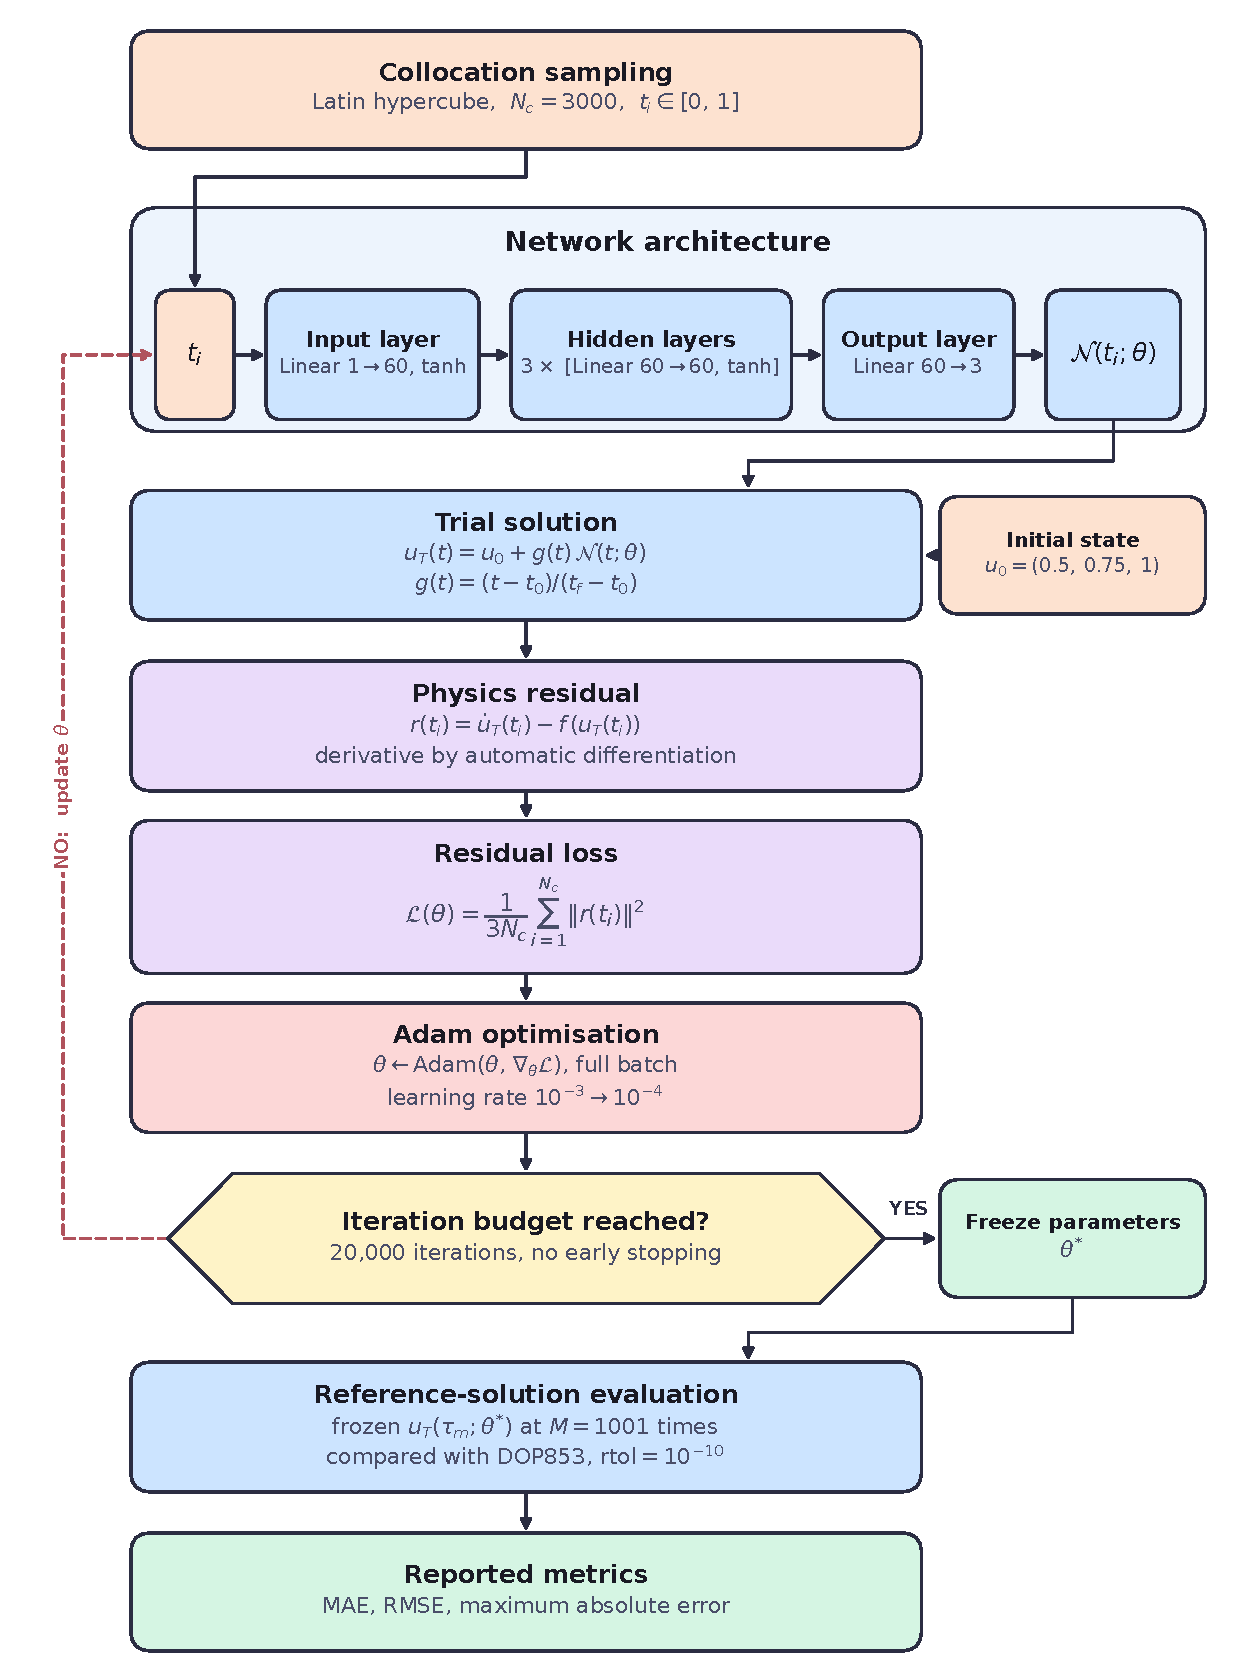
\includegraphics[width=\textwidth]{figures/fig_4_1_pinn_architecture.pdf}
\caption{Constructed pipeline of the Lorenz-1960 PINN.}
\label{fig:pinn_impl_arch}
\end{figure}

In this construction, the data term is empty, and the initial condition is imposed in construction through a trial solution. Weights use Xavier uniform initialization and biases start at zero.

\begin{lstlisting}[caption={Network construction. Depth, width, and activation come from \texttt{Config}, so the architecture is data rather than code.}, label={lst:mlp}]
act = _ACT[cfg.activation]                       # {"tanh": nn.Tanh, ...}
layers = [nn.Linear(1, cfg.width), act()]        # hidden layer 1
for _ in range(cfg.depth - 1):
    layers += [nn.Linear(cfg.width, cfg.width), act()]   # hidden layers 2..4
layers.append(nn.Linear(cfg.width, 3))           # linear output, (x, y, z)
self.net = nn.Sequential(*layers)

for m in self.net:
    if isinstance(m, nn.Linear):
        nn.init.xavier_uniform_(m.weight)
        nn.init.zeros_(m.bias)
\end{lstlisting}

 Listing~\ref{lst:mlp} builds the network, running the loop \texttt{depth - 1} times because the first hidden layer is constructed separately to take the single input feature.

 The initial condition is enforced using a trial solution and the following section explains how it was implemented. 

\section{Enforcing the Initial Condition}
\label{sec:impl_ic}

The initial condition is enforced structurally through a trial solution instead of learning, so training never spends computation on it. Building on the work of Lagaris et al.\ \cite{lagaris1998ann} and Babni et al.\ \cite{babni2025error}, the solution to the candidate is:

\begin{equation}
u_T(t) = u_0 + g(t)\,\mathcal{N}(t;\theta), \qquad g(t) = \frac{t - t_0}{t_f - t_0},
\label{eq:trial}
\end{equation}

where, $\mathcal{N}(t;\theta)$ represents the output of the raw network (Section~\ref{sec:impl_network}). Since  $t_0=0$ and $t_f=1$, the function becomes $g(t)=t$. Therefore, the equality $u_T(t_0) = u_0$ holds for any $\theta$.
Here the subscript $T$ in $u_T(t)$ means \emph{trial}.
The initial condition is enforced and satisfied to machine precision from the start, and cannot degrade during training. 

\begin{lstlisting}[caption={The forward pass, implementing Equation~\ref{eq:trial}.}, label={lst:forward}]
def forward(self, t: Tensor) -> Tensor:
    n = self.net(t)
    if self.ic == "hard":
        g = (t - self.t0) / (self.tf - self.t0)
        return self.u0 + g * n
    return n
\end{lstlisting}

A soft initial condition alternative is implemented through \texttt{Config(ic="soft")}. It follows the initial condition penalty term with coefficient $\lambda_{\mathrm{IC}}$, which needs to be tuned so that the two loss terms continue to be comparable, and it was added by Raissi et al.\ \cite{raissi2019pinn}. This hyperparameter is removed during the hard construction. All the results below refer to the hard construction.

The trial solution now enforces the net to satisfy the initial condition for every parameter. Now we need the model/net to agree on the Lorenz system equations ($\dot{u}_T$ agrees with
$f(u_T)$), Section~\ref{sec:impl_residual} breaks down the equation enforcement in the model through residuals at each collocation point.

\section{The Physics Residual}
\label{sec:impl_residual}

The residual is a measure of how far the candidate is from a solution of the equations:

\begin{equation}
r(t) = \frac{du_T}{dt} - f\big(u_T(t)\big),
\label{eq:residual}
\end{equation}

The residuals are zero when $u_T$ is exact. The derivative is derived from automatic differentiation, and which makes it the exact up to the floating-point precision. A finite-difference estimate would be followed by a truncation error near $10^{-6}$, which is similar to the desired accuracy, and would pollute the value of the quantity to be minimized.

Listing~\ref{lst:residual} is the only place where \texttt{ode\_residual} appears. It takes in the coefficient vector $c$ as an argument, which comes from \texttt{Config.coefficients}. The corresponding terms of the Equation~\ref{eq:impl_lorenz_reduced} are the products \texttt{y*z}, \texttt{x*z}, and \texttt{x*y}. 

\begin{lstlisting}[caption={The residual of Equation~\ref{eq:residual}, and the RHS it subtracts.}, label={lst:residual}]
def residual(model: PINN, t: Tensor) -> Tensor:
    u = model(t)                                  # trial solution, Eq. 4.6
    cols = [torch.autograd.grad(u[:, j].sum(), t,
                                create_graph=True)[0][:, 0]
            for j in range(u.shape[1])]           # d/dt of each component
    dudt = torch.stack(cols, dim=1)
    return ode_residual(u, dudt, model.coeffs)

def ode_residual(u: Tensor, dudt: Tensor, coeffs) -> Tensor:
    c = torch.as_tensor(coeffs, dtype=u.dtype, device=u.device).reshape(3)
    x, y, z = u[:, 0], u[:, 1], u[:, 2]
    f = torch.stack([c[0] * y * z,                # dx/dt = -0.10 y z
                     c[1] * x * z,                # dy/dt =  1.60 x z
                     c[2] * x * y], dim=1)        # dz/dt = -0.75 x y
    return dudt - f
\end{lstlisting}

In line 4, the argument \texttt{create\_graph=True} keeps $\dot{u}_T$ inside the auto-grad graph. Without keeping it, the derivative becomes constant. As a result, the optimizer can't back-propagate to reach $\theta$ through the residual. 
Equation~\ref{eq:residual} defines $r(t)$ at every $t$ in the interval. But training can only be possible in finitely many instants in the interval. Section~\ref{sec:impl_collocation} fixes this issue using collocation points. 

\section{Collocation Points}
\label{sec:impl_collocation}


The residual is enforced at $N_c = 3000$ instants $\{t_i\}_{i=1}^{N_c} \subset [t_0, t_f]$, randomly drawn and fixed in advance of training. The $N_c = 3000$ collocation points are used during the training and  $M=1001$ separate uniformly spaced points are used only to evaluate the model against the baseline. Both sets are in between $[0,1]$, so their different size are intentional. They are obtained from Latin hypercube sampling, which randomly selects a point in each of $N_c$ bins that divide the interval into equal-length subintervals. The drawback of this is that it causes clusters when using a uniform grid and a gap that is more than a bin wide when using an irregular grid; using Latin hypercube sampling solves it.


\begin{lstlisting}[caption={Generating the collocation grid. The sample comes from the unit interval then it was affinely mapped to the solution interval.}, label={lst:collocation}]
def make_grid(cfg: Config, device: torch.device) -> Tensor:
    t0, tf = cfg.t_span
    sample = qmc.LatinHypercube(d=1, seed=cfg.seed).random(cfg.n_collocation)
    t = t0 + (tf - t0) * sample                  # unit sample -> [t0, tf]
    return torch.as_tensor(t, dtype=torch.float32,
                           device=device).reshape(-1, 1)
\end{lstlisting}

The training is full batch, with all iterations evaluating the residuals, and no noise in the gradient arriving at any of the mini-batches.

Residuals in a finite set of instants are now available and Section~\ref{sec:impl_training} explains how we combine them into a single number that the training minimizes to learn. 

\section{Loss Function and Training Protocol}
\label{sec:impl_training}

The objective, or mean squared residual at the collocation points,

\begin{equation}
\mathcal{L}(\theta) = \frac{1}{3N_c} \sum_{i=1}^{N_c} \big\| r(t_i) \big\|^2 .
\label{eq:loss}
\end{equation}

The network is optimized with respect to these equations and if it is used alone, then the path it traces is determined by the residuals and an initial condition that was hard-wired into Equation~\ref{eq:trial}. The present implementation is different from the data-driven formulation of Chapter~2.

The number of optimization iterations with Adam is set to $20{,}000$, while the learning rate decays linearly from $10^{-3}$ to $10^{-4}$. The loop is listed in~\ref{lst:train}. The collocation grid is duplicated for every iteration because the tensor used to differentiate \texttt{requires\_grad\_} marks and the graph is discarded at the end of every back pass.

\begin{lstlisting}[caption={The training loop. \texttt{LambdaLR} on line 3 is linear interpolation started from the beginning and end learning rates across the entire budget.}, label={lst:train}]
adam = torch.optim.Adam(model.parameters(), lr=cfg.lr_start)
decay = cfg.lr_end / cfg.lr_start
sched = torch.optim.lr_scheduler.LambdaLR(
    adam, lambda e: 1.0 + (decay - 1.0) * min(e, cfg.epochs) / cfg.epochs)

for epoch in range(cfg.epochs):
    adam.zero_grad()
    res, ic = loss_terms(model, grid.clone().requires_grad_(True))
    loss = res + model.gamma * ic if cfg.ic == "soft" else res
    loss.backward()
    adam.step()
    sched.step()
\end{lstlisting}

The complete configuration is given in Table~\ref{tab:pinn_hyper}. An L-BFGS polishing stage is included in \texttt{train.py}. It also disables  \texttt{lbfgs\_iters = 0}, and therefore the results below are from Adam alone.

\begin{table}[H]
\centering
\caption{Training configuration for the reported run.}
\label{tab:pinn_hyper}
\begin{spacing}{1.0}
\small
\begin{tabular}{|l|l|l|l|}
\hline
\textbf{Setting} & \textbf{Value} & \textbf{Setting} & \textbf{Value} \\
\hline
Layers $\times$ width & $4 \times 60$ & Optimizer & Adam, full batch \\
\hline
Activation & tanh & Iterations & $20{,}000$ \\
\hline
Parameters & $11{,}263$ & Learning rate & $10^{-3}$ to $10^{-4}$, linear \\
\hline
Collocation points & $3000$, Latin hypercube & Precision & single (float32) \\
\hline
Initial condition & hard, Equation~\ref{eq:trial} & Random seed & $0$ \\
\hline
\end{tabular}
\end{spacing}
\end{table}

The architecture and the optimizer settings are taken from Section 4.1 of the reference study \cite{matthews2024pinnde}, which numerically solves the Euler rigid-body equations using PINN. Its Section 4.2, the source of the following solution to that system by a deep operator network, presumably done by the Lorenz-1960 equations. A multi-layer feed-forward network with four hidden layers of $40$ neurons each; soft initial conditions, $5000$ sampled initial conditions; and $75{,}000$ iterations. The following configuration is not found in any one of the experiments in that study, which is relevant to the interpretation of Section~\ref{sec:impl_comparison}.

Training is now fully specified and can be reproduced. Now we need to measure the trained network against the reference solution of Section~\ref{sec:impl_reference}.


\section{Model Evaluation}
\label{sec:impl_evaluation}

Training and evaluation are two vital phases of this research. There is no overlap between training and evaluation. The final iteration's parameters are frozen and stored. There were no early stops, and we selected the weights from the final iteration. The trained model is then evaluated against $M = 1001$ times $\{\tau_m\}$ of Section~\ref{sec:impl_reference}, here $\tau_m$ denote the $m$-th time of the evaluation grid. The model was not evaluated using the collocation points $\{t_i\}$ it was trained on.

\begin{lstlisting}[caption={The evaluation pass, abridged from \texttt{train.py}. The metrics of Table~\ref{tab:pinn_metrics} come from line 3.}, label={lst:evaluate}]
t, ref = reference_trajectory(cfg, n=1001)  # the evaluation grid
pred = predict(model, t)                    # frozen weights, no gradient
metrics = compute_error_metrics(ref, pred)  # MAE, RMSE, max |error| per state
metrics.to_csv(cfg.results_path / "metrics.csv", index=False)
\end{lstlisting}

\texttt{compute\_error\_metrics} uses the same three quantities for each state and for the correct one.
The sum of all the elements in Table~\ref{tab:pinn_metrics} is, known as the Euclidean norm of the error vector. The root mean squared error between the actual trajectory and the DOP853 trajectory, and the pointwise residual of Equation~\ref{eq:residual} over the interval. No evaluation time comes into the loss. No collocation time will be used in the metrics of Equation~\ref{eq:loss}. Section~\ref{sec:impl_results} reports the
numbers and the figures of training behavior and the solution.



\section{Results}
\label{sec:impl_results}

This section reports the performance of the trained network under the measures of Section~\ref{sec:impl_evaluation}. The error is calculated against the reference shown in Section~\ref{sec:impl_results_metrics}. And then is shown the solution, training behind it, and pointwise residuals are shown in detail with figures in Section~\ref{sec:impl_results_figures}. 

Over the time interval  $[0, 1]$ the trajectory moves from $(x, y, z) = (0.5, 0.75, 1.0)$ to $(0.412, 1.359, 0.631)$

\subsection{Error Metrics}
\label{sec:impl_results_metrics}

Table~\ref{tab:pinn_metrics} reports the error over the full $1001$-point grid. The combined row is the Euclidean magnitude of the three-component error vector, not an average.

\begin{table}[H]
\centering
\caption{Error of the trained PINN against the DOP853 reference over $1001$ points.}
\label{tab:pinn_metrics}
\begin{spacing}{1.0}
\small
\begin{tabular}{|l|l|l|l|}
\hline
\textbf{State} & \textbf{MAE} & \textbf{RMSE} & \textbf{Max. abs. error} \\
\hline
$x$ & $5.20 \times 10^{-6}$ & $5.77 \times 10^{-6}$ & $9.24 \times 10^{-6}$ \\
\hline
$y$ & $1.12 \times 10^{-5}$ & $1.36 \times 10^{-5}$ & $2.56 \times 10^{-5}$ \\
\hline
$z$ & $8.27 \times 10^{-6}$ & $9.04 \times 10^{-6}$ & $1.25 \times 10^{-5}$ \\
\hline
Combined $L_2$ & $1.66 \times 10^{-5}$ & $1.73 \times 10^{-5}$ & $2.60 \times 10^{-5}$ \\
\hline
\end{tabular}
\end{spacing}
\end{table}

Against states spanning $0.41$ to $1.36$, an error near $10^{-5}$ is close to five correct decimal. Without the network seeing any value of the solution, digits were retrieved. The largest errors fall in $y$, the state with the widest range and the largest coefficient.

\subsection{Solution and Training Behaviour}
\label{sec:impl_results_figures}

The trained solution is plotted against the reference in Figure~\ref{fig:solution}. All three states are smooth and monotone on $[0, 1]$: $x$ falls from $0.5$ to $0.412$, $y$ rises from $0.75$ to $1.359$, and $z$ falls from $1$ to $0.631$.

\begin{figure}[H]
\centering
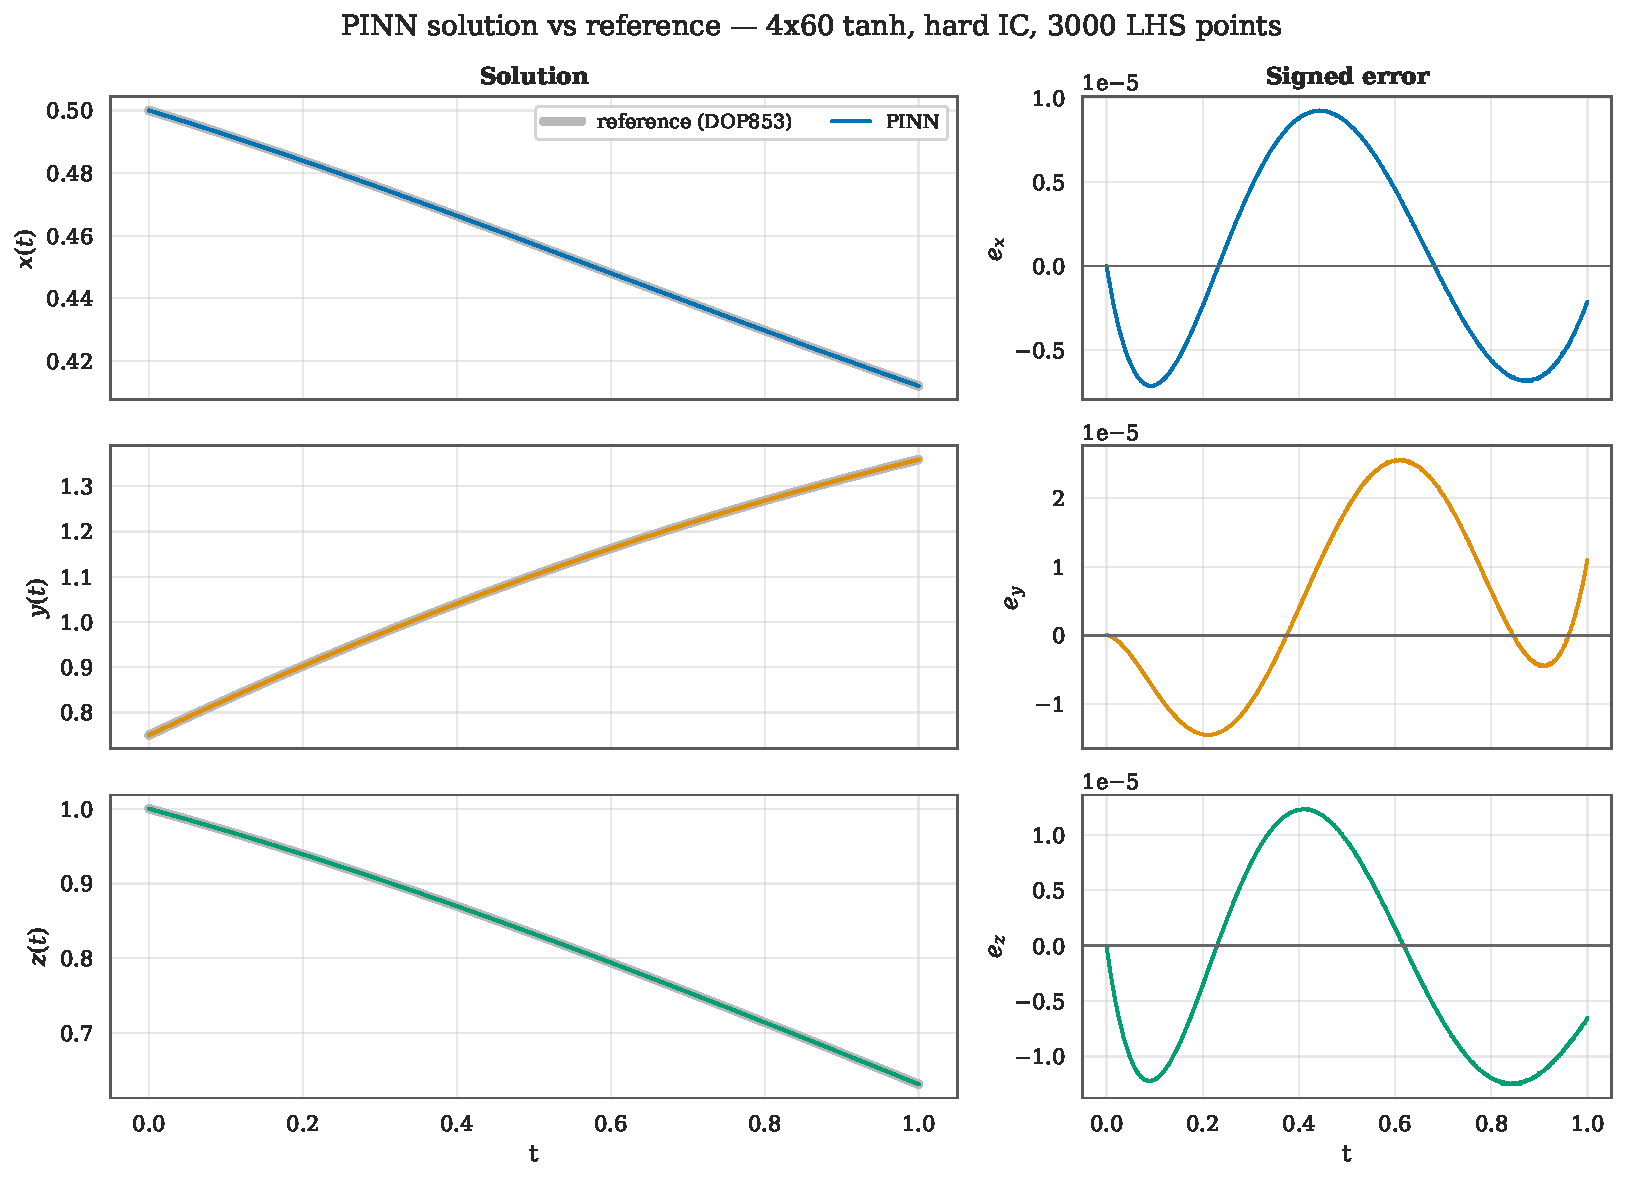
\includegraphics[width=0.85\textwidth]{figures/fig_4_2_solution_vs_reference.pdf}
\caption{PINN solution against the reference for each state, with the signed error beside each panel.}
\label{fig:solution}
\end{figure}

The training loss falls from $2.17 \times 10^{-1}$ to $6.82 \times 10^{-9}$ over the run, eight orders of magnitude. Also, there is no plateau or divergence.

\begin{figure}[H]
\centering
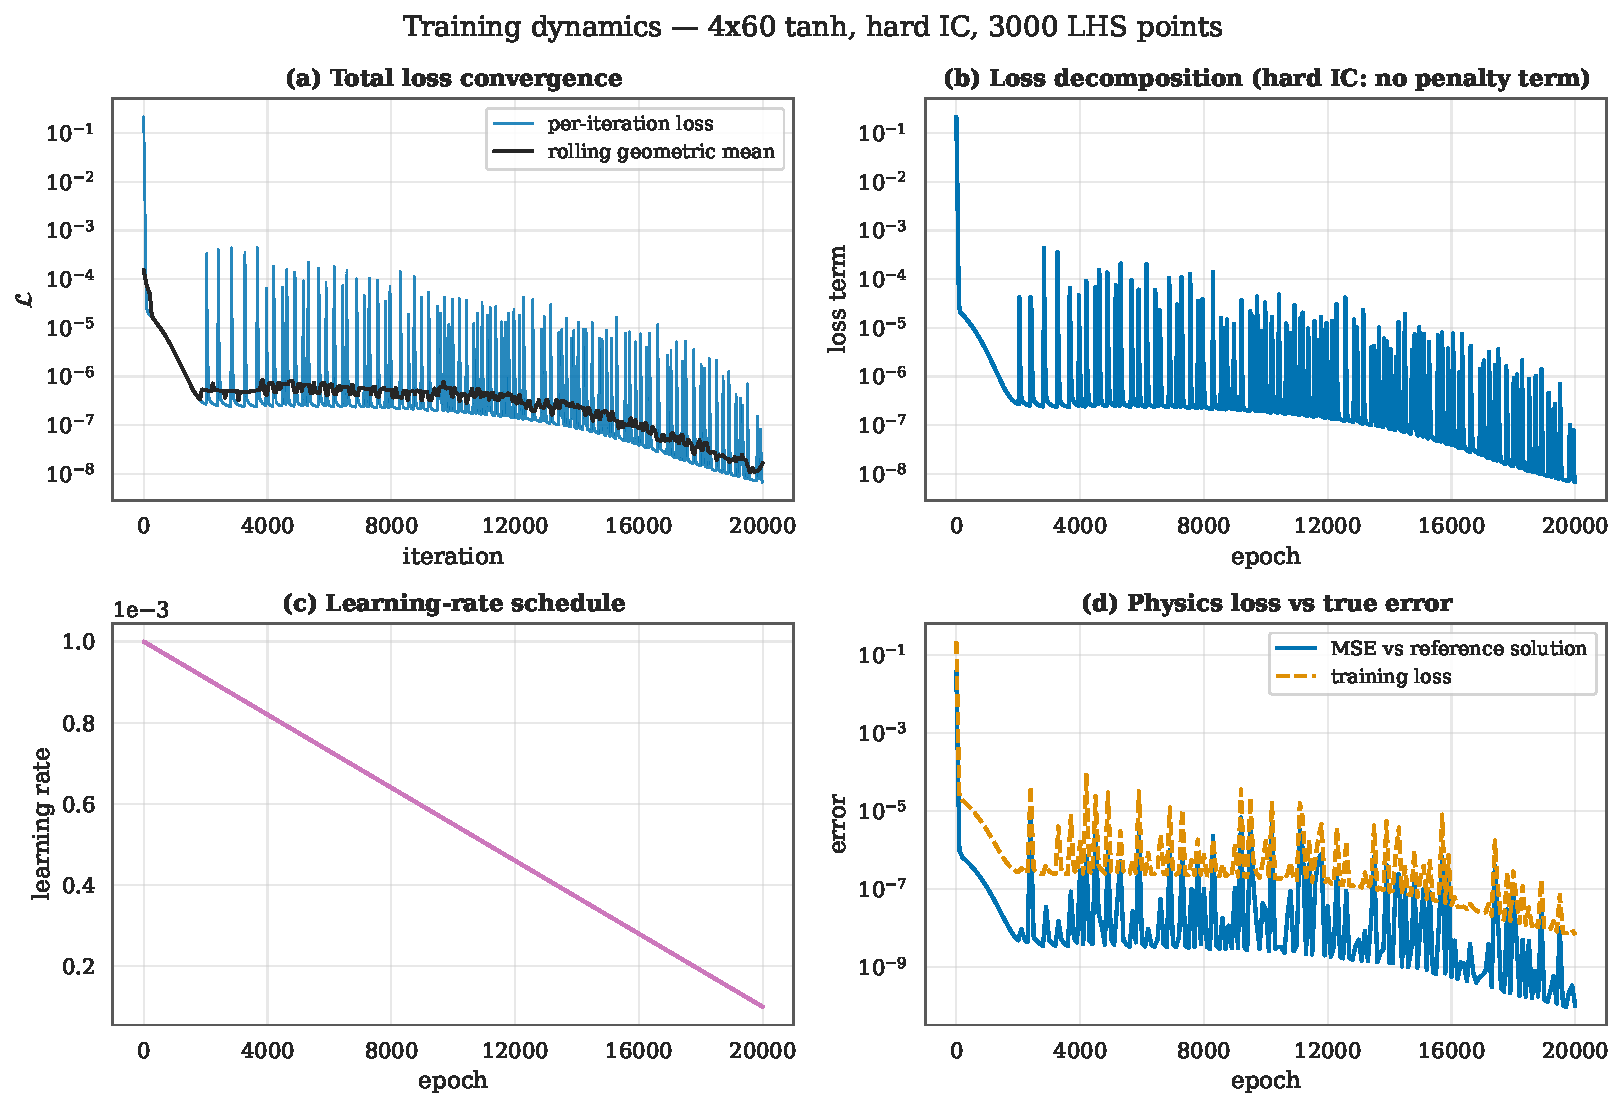
\includegraphics[width=0.80\textwidth]{figures/fig_4_3_training_dynamics.pdf}
\caption{Loss convergence, loss decomposition, learning-rate schedule, and reference error sampled every $100$ iterations.}
\label{fig:training}
\end{figure}

When a small average loss is obtained, the equations do not necessarily hold everywhere. Figure~\ref{fig:residual} shows the residual across the interval and confirms that they hold uniformly across the interval rather than in an average sense.

\begin{figure}[H]
\centering
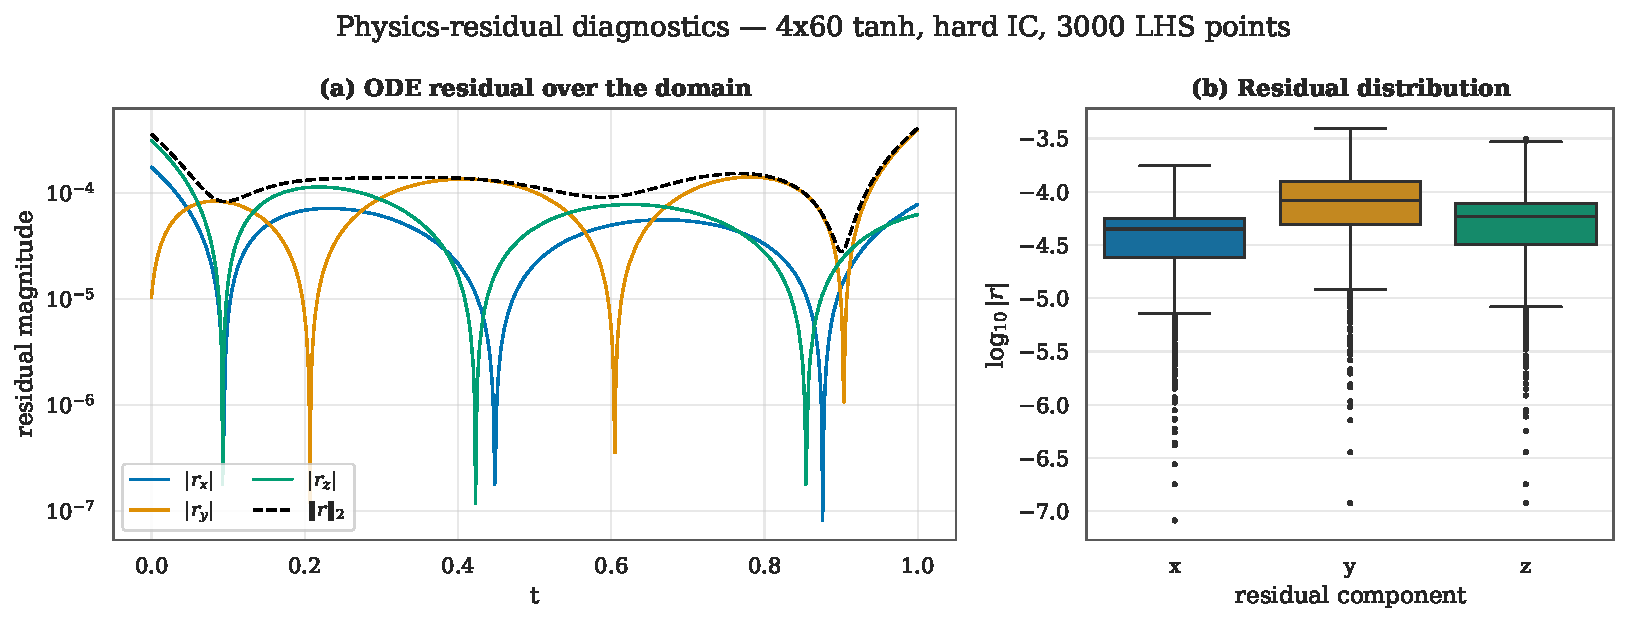
\includegraphics[width=0.80\textwidth]{figures/fig_4_4_physics_residual.pdf}
\caption{Magnitude of the ODE residual across the solution interval for the trained network.}
\label{fig:residual}
\end{figure}

\section{Comparison with the Reference Study}
\label{sec:impl_comparison}

Matthews and Bihlo \cite{matthews2024pinnde} present their Lorenz-1960 result as figures: the solution, the difference from a Runge-Kutta reference, and the training loss. They state that they use mean squared error as their metric, and they do not provide an error value table for this system. There is no direct numerical comparison to make, and no attempt is made to make such a comparison.  They have a difference plot that is consistent in order of magnitude with the data in Table~\ref{tab:pinn_metrics}, which is as much as a published figure supports.

Both designs are shown side by side in Table~\ref{tab:method_comparison}. The four settings vary, and any reading of the accuracy figures must account for all four. 

\begin{table}[H]
\centering
\caption{Method design compared with the reference study's Lorenz-1960 experiment.}
\label{tab:method_comparison}
\begin{spacing}{1.0}
\small
\begin{tabularx}{\textwidth}{|p{3.6cm}|>{\raggedright\arraybackslash}X|>{\raggedright\arraybackslash}X|}
\hline
\textbf{Aspect} & \textbf{\cite{matthews2024pinnde}, Sec.~4.2} & \textbf{This work} \\
\hline
Model class & Deep operator network & Physics-informed network \\
\hline
Layers $\times$ width & $4 \times 40$ & $4 \times 60$ \\
\hline
Initial condition & Soft, penalty in the loss & Hard, by trial solution \\
\hline
Initial conditions sampled & $5000$, over $[-2,2]^3$ & One, the benchmark value \\
\hline
Training iterations & $75{,}000$ & $20{,}000$ \\
\hline
What is learned & The solution operator $G(u_0)(t)$ & One trajectory $u(t)$ \\
\hline
Reported accuracy & Figures only & Table~\ref{tab:pinn_metrics} \\
\hline
\end{tabularx}
\end{spacing}
\end{table}

These two methods are addressing different questions. An operator network learns a mapping from initial conditions to solutions, a harder problem that explains both its larger budget and its soft constraints. The PINN here learns one trajectory, and the hard initial condition is available precisely because that trajectory is fixed in advance. The error table shown above appears to be the first published table of the numerical accuracy of a physics-informed solution of this system at these parameters.

\chapter{Standards and Design Constraints}


\section{Compliance with the Standards}



\section{Design Constraints}


\section{Cost Analysis}


\section{Complex Engineering Problem}

This project is a complex engineering problem. It is not just writing code. We need to understand math, build numerical solvers, design neural networks, and compare results carefully. The Lorenz-1960 system is nonlinear and coupled, so solving it with an ANN requires real engineering decisions, not just running a script.

\subsection{Complex Problem Solving}

Table~\ref{tab:p_solve} shows how this project maps to the complex problem solving categories.

\begin{center}
    \begin{table}[ht]
        \centering
        \caption{Mapping with complex problem solving.}
        \begin{tabular}{|p{0.12\textwidth}|p{0.12\textwidth}|p{0.12\textwidth}|p{0.12\textwidth}|p{0.12\textwidth}|p{0.12\textwidth}|p{0.12\textwidth}|}
        \hline
        P1& P2& P3& P4& P5& P6& P7\\
        Dept of Knowledge & Range of Conflicting Requirements & Depth of Analysis & Familiarity of Issues & Extent of Applicable Codes & Extent of Stakeholder Involvement & Inter-dependence\\
        \hline 
        $\checkmark$ & $\checkmark$ & $\checkmark$ & $\times$ & $\times$ & $\times$ & $\checkmark$\\
        &&&&&&\\
        \hline 
        \end{tabular}
        \label{tab:p_solve}
    \end{table}
\end{center}

\subsubsection{P1: Depth of Knowledge ($\checkmark$)}

Many things are needed to be known at once: how ODEs work, how numerical solvers like Runge-Kutta produces reference solutions, how the neurons learn, how optimizers such as Adam update the weights, and how to measure errors. One of these isn't sufficient. All are linked together.

\subsubsection{P2: Range of Conflicting Requirements ($\checkmark$)}

We face trade-offs. A larger network could yield higher accuracy at the cost of training time.
and may overfit. A more quickly trained system might be unstable. A model that performs really well the first time around may not be able to run with a different random number seed. We can't have it all at the same time. so, we have to find a good balance.


\subsubsection{P3: Depth of Analysis ($\checkmark$)}

We don't simply execute the code and see if it is working. We tested several ANN configurations and observe that: Understand the meaning of the error numbers, observe the behavior of training, determine whether results converge, and why One configuration is better than the other. It's the real analysis.

\subsubsection{P4: Familiarity of Issues ($\times$)}

This Lorenz-1960 system is a well-known benchmark and the methods we have been using, such as Runge-Kutta solvers, feedforward ANNs, Adam optimizer are all established. Although
While our specific combination is new, the issues that are not new to practitioners.Thus this criterion is not applicable.


\subsubsection{P5: Extent of Applicable Codes ($\times$)}

Our project is a computational research study, not a commercial or safety critical system.We are not currently subject to any industry standards, regulations or professional codes which limit the ways in which we
Design and test the accuracy of the ANN. Thus, this criterion is not valid.


\subsubsection{P6: Extent of Stakeholder Involvement ($\times$)}

Only student researchers and academic supervisors are stakeholders.There are no external clients/end-users/regulatory bodies whose conflicting needs need to be
balanced.All decisions are made on the basis of science, not stakeholder demands.So this doesn't applicable for criterion.


\subsubsection{P7: Interdependence ($\checkmark$)}

All of the components of this project are interrelated. The solver makes the training data.The data influences the learning process of the ANN. The results are dependent on the ANN design. The optimizer affects training. Just one part goes wrong, the whole result is impacted.



\subsection{Engineering Activities}

Table~\ref{tab:e_act} shows how this project maps to the complex engineering activity categories.

\begin{center}
    \begin{table}[ht]
        \centering
        \caption{Mapping with complex engineering activities.}
        \begin{tabular}{|p{0.18\textwidth}|p{0.18\textwidth}|p{0.18\textwidth}|p{0.18\textwidth}|p{0.18\textwidth}|}
        \hline
        A1& A2& A3& A4& A5\\
        Range of resources & Level of Interaction & Innovation & Consequences for society and environment & Familiarity\\
        \hline 
        $\checkmark$ & $\checkmark$ & $\checkmark$ & $\times$ & $\checkmark$\\
        &&&&\\
        \hline 
        \end{tabular}
        \label{tab:e_act}
    \end{table}
\end{center}

\subsubsection{A1: Range of Resources ($\checkmark$)}

We utilise many different tools and sources of knowledge: ODE math, Runge-Kutta solvers, SciPy, PyTorch, NumPy, Matplotlib and 13 research papers. There are no single tools or information source which can handle all this. This is sufficient to complete this project.



\subsubsection{A2: Level of Interaction ($\checkmark$)}

This project talk is an on-going dialogue between parts. The data is fed to the ANN by the solver. The ANN design affects training. Training configuration impacts on outcomes. The assessment is based on
everything before it. One cannot work on one aspect without taking into consideration the others.


\subsubsection{A3: Innovation ($\checkmark$)}
A systematic comparison of the architecture of plain ANNs on Lorenz-1960 system has.
This is the first time this system has not been performed. Most of the current works are based on PINNs or
hybrid approaches \cite{matthews2024pinnde}. We pose a new question: is it feasible for a simple ANN with no supervision or feedback to do this?
Is it still possible to do a good job on this using physics in the loss function? This is the new section.



\subsubsection{A4: Consequences for Society and Environment ($\times$)}

Our project is a purely academic study which is training small networks on its own computer.Computer Does not create any physical product, does not impact public health or is
safe and requires little computational resources. The Lorenz-1960 system is a theoretical.
We are not benchmarking and are not going to make any real world choices based on our results. This criterion is not applicable.



\subsubsection{A5: Familiarity ($\checkmark$)}
This is NOT a textbook type problem. The Lorenz-1960 system is a nonlinear system and chaotic. This is not a pre-made ANN setup that we can just use. We will need to
Let's learn by doing, determine the best architecture for our purpose and be careful to understand. when the training loss is low, this doesn't mean that the solution is what it is.
is right everywhere.



\subsection{Knowledge and Attitude Profile}

Table~\ref{tab:k_profile} shows how this project maps to the knowledge and attitude profile categories.

\begin{center}
    \begin{table}[ht]
        \centering
        \caption{Mapping with knowledge and attitude profile.}
        \begin{tabular}{|p{0.08\textwidth}|p{0.08\textwidth}|p{0.08\textwidth}|p{0.08\textwidth}|p{0.08\textwidth}|p{0.08\textwidth}|p{0.08\textwidth}|p{0.08\textwidth}|p{0.08\textwidth}|}
        \hline
        WK1& WK2& WK3& WK4& WK5& WK6& WK7& WK8& WK9\\
        Natural Sciences & Math \& Analysis & Eng. Funda- mentals & Specialist Knowledge & Resource Use & Eng. Practice & Role in Society & Research Lit. & Ethics\\
        \hline 
        $\checkmark$ & $\checkmark$ & $\checkmark$ & $\checkmark$ & $\times$ & $\checkmark$ & $\times$ & $\checkmark$ & $\checkmark$\\
        &&&&&&&&\\
        \hline 
        \end{tabular}
        \label{tab:k_profile}
    \end{table}
\end{center}

\subsubsection{WK1: Natural Sciences ($\checkmark$)}

We need to have a good knowledge of the natural sciences, particularly physics, in our project.
The Lorenz-1960 system is a meteorological model which illustrates atmospheric convection. Understanding of the theory of nonlinear coupled.To accurately model these physical phenomena, ODEs are required.


\subsubsection{WK2: Mathematics and Numerical Analysis ($\checkmark$)}

The mathematics and numerical analysis are heavily used in this project and are conceptually based. We use advanced calculus for ODEs, Runge-Kutta method to have reference numerical solutions and statistics to calculate mean squared error of our ANN predictions.The key interest in evaluating training convergence and model accuracy is data analysis.


\subsubsection{WK3: Engineering Fundamentals ($\checkmark$)}

We use a structured approach to engineering principles using a clearly defined formulating a problem mathematically and solving it by computer. The translation of the Lorenz-1960 mathematical equations into a computational model is what was called the process.Involves using core engineering methodology.


\subsubsection{WK4: Specialist Knowledge ($\checkmark$)}

Our research is on the cutting edge of the field and focuses on the possibilities of artificial application of neural networks to the solution of a complex system of ODEs. This requires specialist engineering knowledge in deep learning models such as PyTorch, optimization algorithms such as Adam,
and network architectures.


\subsubsection{WK5: Engineering Design (Sustainability) ($\times$)}

This project is a theoretical mathematical benchmark study which is computational research. It is not using of physical resources, environmental impact assessments or whole-life cost considerations. Hence this criterion is not applicable.


\subsubsection{WK6: Engineering Practice (Technology) ($\checkmark$)}

We extensively use modern engineering practice and technology. We utilize programming languages and scientific computing libraries (SciPy, NumPy, Matplotlib) that are standard practice in the field of computational engineering and data science.

\subsubsection{WK7: Role of Engineering in Society ($\times$)}

The Lorenz-1960 system benchmark is not directly related to public safety, societal issues, or the use of information technology in the nation. or sustainable development. It's a scholarly exercise of algorithm assessment then, There are no direct societal stakeholders whose safety is to be taken into account. This criterion does not apply.


\subsubsection{WK8: Engagement with Research Literature ($\checkmark$)}

To gain insight into how we are expected to act, we did extensive literature review many research papers. The latest advancements in PINNs and conventional ANNs for solving ODEs. We applied No prior studies have explored how the performance of plain ANNs can be assessed on the The Lorenz-1960 system that does not include physics-informed loss functions.

\subsubsection{WK9: Ethics and Professional Conduct ($\checkmark$)}

Following the practice of professional ethics and academic integrity, all research is properly cited. For papers and methodologies these were used. Our experiments are reproducible and our Results are presented truthfully and not manipulated.



\section{Summary}
\chapter{Conclusion}

The present work investigates whether the same concept of copying the solution of an ordinary differential equations system, as was done for the Lorenz-1960 set, can be applied to the simple feedforward artificial neural network with a much lower accuracy of the reference data, which is in the form of numerical data. Motivation is practical and academic tension. There are classical numerical solvers like Runge-Kutta methods that provide dependable reference solutions, but they solve the system step by step on a fixed grid. A continuous input/output mapping can be learned over time by neural approaches. Although PINNs have been introduced for the solution of differential equations in recent efforts, state variables are still relevant classes of variables. Losses, or operator-learning architectures \cite{matthews2024pinnde, babni2025error, lau2020oden}. This study thus focuses on narrows. The data-driven feedforward ANN is trained to approximate $(x(t), y(t), z(t))$ for the Lorenz-1960 initial value problem, without adding ODE residual terms to the loss function.

The research design is controlled architecture comparison with validated numerical baseline. The parameters for the Lorenz-1960 formulation, initial conditions and time. The system used in the reference problem of Chapter 2 (PinnDE) is used in the intervals. Two numerical solvers are used to produce the reference trajectory and to validate it. The reference trajectory is generated and validated with a custom numerical solver, as well as a commercial numerical solver. RK4 is applied before using it as training data and SciPy DOP853 is used. The ANN study is divided into two parts. In phase 1 the depth, width and optimizer are kept constant and the activation function is changed. During the first phase the depth, width and optimizer are fixed and the activation function is changed. Phase 2 compares Adam, L-BFGS and SGD with momentum on the top-performing phase 1 architectures. This separation is made to make the interpretation of the architecture and optimiser effects easier. The predicted result of the work will be an empirical benchmark to make an approximation of the Lorenz-1960 system to a simple ANN. Previous works have shown that neural networks are able to solve, or to approximate, differential equations of a wide range of formulations \cite{mall2013comparison, okereke2021novel, dubey2024solving}. The physics-informed approaches have been used for Lorenz-type problems  \cite{matthews2024pinnde, aslam2024neuro}. The academic merit of this project is that it is based on the simpler and more straightforward question of how far a standard feedforward ANN can be pushed by systematic variations in its architecture and an exploration of the results it learns. A verified numerical solution is called a training target. The solution can help determine if the bracelet is or is not better. What about the physics informed constraints, is it required for this benchmark or can plain-ANN design be used? These are still necessary to get a higher accuracy and reliability. At this report stage the supported contribution is: The validated baseline design, the dataset and training protocol, and the planned evaluation framework. If the experiment records the declaration of a final best ANN architecture then the report does not state a final best ANN architecture. In Chapter 4, you will find metric tables and plots. This is intentional. Without supporting evidence, any claim of accuracy would detract from the study. Final conclusions regarding the optimal depth, width, activation function or optimizer should be finalized only after careful experimental research and analysis. Planned comparison is completed and research needs to be continued in the study. Three directions. First, the most suitable configuration needs to be tested repeatedly over random Use of seeds to check for stability. Second, in order to assess the generalization of the trained model, it needs to be tested on denser Use time grids or other initial conditions. Third, the ANN results obtained in the plain should be compared with the physics-based, literature informed and operator learning baselines in a more direct manner. These extensions would assist in deciding if the architecture chosen for this project is effective for only one or more of the objects, controlled trajectory or for wider neural approximation of nonlinear ODE systems.



\bibliographystyle{unsrt}
\bibliography{fydp}
\addcontentsline{toc}{chapter}{References}

\clearpage
%\appendix 

%\phantomsection

%\addcontentsline{toc}{chapter}{Appendices}
%\chapter{Amino Acids\label{appAmino}}
%\begin{figure}[h]
%\begin{center}
%\includegraphics[width=1\textwidth]{./images/background/aminoacids}
%\end{center}
%\caption{Twenty different amino acids, their structures and chemical properties.\index{Amino Acid!chemical properties}\cite{Lehninger2012}.}
%\end{figure}
%\clearpage
%\thispagestyle{empty}
%\mbox{}

%\clearpage
%\phantomsection
%\addcontentsline{toc}{chapter}{Index}
%\printindex

\end{document}
